%\documentclass[a4paper,12pt,oneside,draft]{report}
\documentclass[a4,12pt,fullpage]{report}
%\setpapersize{A4}
%\usepackage{a4}
%\usepackage{lscape} % in latex preamble
\usepackage{amssymb,graphicx, rotating, epstopdf}
\usepackage{epsfig,amsmath,amsfonts}
\usepackage{float}
\usepackage[english]{babel}
\usepackage{subfigure}
\usepackage{vmargin}
\usepackage{textcomp}
\usepackage{notebook}
\usepackage{setspace}
\usepackage{pxfonts}
\usepackage{booktabs}
\usepackage{mathtools}
\usepackage{amsmath}
\usepackage{amssymb}
\usepackage{cancel}
\usepackage{subfigure}
\usepackage[export]{adjustbox}
    \usepackage{wrapfig, framed,multicol}
    \usepackage{lipsum}
    \usepackage{filecontents}
    \usepackage[numbered,framed]{matlab-prettifier}%

        % Line spacing
%\setmargins{3.5cm}{3.5cm}{14cm}{20cm}{0pt}{2cm}{0pt}{3cm}
%\setmargins{2.5cm}{2.5cm}{16cm}{22cm}{0pt}{1cm}{0pt}{2cm}
%\usepackage{showkeys}
\usepackage{fancyhdr}
%\pagestyle{fancy}
%\lhead{\nouppercase{\leftmark}}
%\chead{}
%\rhead{\thepage}
%\lfoot{}
\newtheorem{thm}{Theorem}[section]
\newtheorem{definition}{Definition}[section]
\newtheorem{remark}{Remark}[section]
\newtheorem{proof}{Proof}[section]
\newtheorem{example}{Example}[section]
\newtheorem{lemma}{Lemma}[section]
%\newtheorem{property}[thm]{Property}
%\definition{def}{Definition}[chapter]
%\cfoot{\thepage}
%\rfoot{}
\topmargin 1cm
\oddsidemargin 2cm
\evensidemargin 2cm
\textwidth 16.59cm
\textheight 21.94cm
\renewcommand{\baselinestretch}{0.5}


%%%%%%%%%%%%%%%%%%%%%%%%%%%%%%%   LAYOUT OF THE THESIS %%%%%%%%%%%%%%%%%%%%%%%%%%
%\input{thesis_layout.tex}
%%%%%%%%%%%%%%%%%%%%%%%%%%%%%%%%% NEW DEFINITIONS       %%%%%%%%%%%%%%%%%%%%%%%%%
%%%%%%%%%%%%%%%%%%%%%%%%%%%%%%%%% MAIN DOCUMENT %%%%%%%%%%%%%%%%%%%%%%%%%%%%%%%%%
%\includeonly{section2}
%\includeonly{ch4}
\begin{document}

\onehalfspacing

%\noindent
%%%%%%%%%%%%%%%%%%%%%%%%%%%%%%%%% TITLE PAGE %%%%%%%%%%%%%%%%%%%%%%%%%%%%%%%%%%%%
%\pagenumbering{roman}
%\setcounter{page}{1}
%\thispagestyle{empty}
\thispagestyle{empty}
\begin{center}
\vspace*{1cm}
{\huge Mathematical Modeling of Cell Signalling Pathways in Cancer: Numerical Investigation and Stability Analysis}

\vspace*{1.5cm}
\large { for the Bachelor of Science (General) Degree \\By\\E.S.K.Chandrasekara\\Sc/2018/10559}\\
\vspace{1.3cm}
\large {Supervisor:\\ Dr. L. W. Somathilake }\\
\vspace{1.9cm}
%\date{Date}
\large{Department of Mathematics}\\
\large{University of Ruhuna}\\
\large{Matara.}\\
\vspace{0.5cm}
\large{2023}
\end{center}





\pagenumbering{roman}
\setcounter{page}{1}
%\newpage
%%%%%%%%%%%%%%%%%%%%%%%%%%%%%%%% ACKNOWLEDGEMENTS ABSTRACT etc.%%%%%%%%%%%%%%%%%%
%\thispagestyle{empty}
\include{dec}
%\noindent
%\newpage
%%%%%%%%%%%%%%%%%%%%%%%%%%%%%%%%  MAIN CHAPTERS %%%%%%%%%%%%%%%%%%%%%%%%%%%%%%%%%
\chapter*{Acknowledgment}
\paragraph{}
 
This project becomes a reality with the kind support and help of many individuals. I would like to extend my sincere thanks to all of them.

First, I would like to express my deepest gratitude to my supervisor, Dr. L. W. Somathilake for his continuous contribution and supervision throughout the completion of this project which was invaluable.

I am extremely thankful to Prof. Leslie Jayasekara, Head of Mathematics Department, for offering us this course to get this opportunity to pursue our degree.

Besides my supervisor, I wish to thank Dr.Pubudu Thilan for conducting previous lectures and offering us Java programming opportunities. Without her passionate participation,
this project could not have been successfully conducted.

I am also thankful to all academic staff members of the Department of Mathematics of the Faculty of Science University of Ruhuna for their kind advice.

An extra special thank you to my group members, who were simply the greatest. 


\chapter*{Abstract}
\paragraph{}

The intracellular signalling network involved in apoptosis is a complex system crucial to regulating cell death. Despite the advancements made in the field of cell signalling, there remain several limitations in our understanding of these pathways. The study focused on analyzing the interactions between the STAT1, STAT3, Bcl-2, and BAX proteins and their impact on the network. This research contributes to the advancement of our understanding of the intracellular signalling network involved in apoptosis and highlights the importance of mathematical modelling approaches in the study of cell signalling. This study focuses on mathematical modeling approaches for cell signalling and aims to understand the genetic alterations in signalling pathways in cancer and their downstream signalling. The project explores the intracellular signalling network of proteins STAT1, STAT3, Bcl-2, and BAX and presents a mathematical model of the apoptosis signalling network. The mathematical model includes ordinary differential equations that govern the intracellular signalling network, and the numerical results were obtained using Euler's method and Runge-Kutta fourth-order method. The results of the study show that there are three equilibrium points when S = 0.4, two of which are stable with AB $<$ 1, while the third is unstable with AB $>$ 1. The results also show that when S = 0, the equilibrium point is stable, and when S = 1, the equilibrium point is also stable with AB $<$ 1. The study concludes with a summary of the findings and recommendations for future research. This study provides valuable insights into the mathematical modeling of cell signalling and how genetic alterations in signalling pathways can impact downstream signalling in cancer. It highlights the importance of mathematical modeling in understanding complex biological systems and provides a foundation for further research in this field.

%\renewcommand{\contentsname}{Contents}  % Original name = Contents
%\chapter*{Acknowledgment}
\paragraph{}
 
This project becomes a reality with the kind support and help of many individuals. I would like to extend my sincere thanks to all of them.

First, I would like to express my deepest gratitude to my supervisor, Dr. L. W. Somathilake for his continuous contribution and supervision throughout the completion of this project which was invaluable.

I am extremely thankful to Prof. Leslie Jayasekara, Head of Mathematics Department, for offering us this course to get this opportunity to pursue our degree.

Besides my supervisor, I wish to thank Dr.Pubudu Thilan for conducting previous lectures and offering us Java programming opportunities. Without her passionate participation,
this project could not have been successfully conducted.

I am also thankful to all academic staff members of the Department of Mathematics of the Faculty of Science University of Ruhuna for their kind advice.

An extra special thank you to my group members, who were simply the greatest. 


%\begin{spacing}{1.5} % Environment for 1.2 line spacing for contents and lists
\tableofcontents
\newpage
%\cleardoublepage
%\end{spacing}
%\begin{spacing}{1.2}
\listoftables
\newpage
\listoffigures
%\cleardoublepage
%\end{spacing}
\newpage
%\addcontentsline{toc}{chapter}{Introduction}
\pagenumbering{arabic}
\setcounter{page}{1}
%\input{chap0.tex}
%\include{Ch2.tex}
 %\chapter{Introduction}
\label{chap:01}


\paragraph{}


 Models in cell biology are both familiar and mysterious. On the one hand, biologists have traditionally utilised models to represent reality, such as diagrams, rules, graphs, plots, chemical formulas, and relationships. Their purpose is to be similar to numerous organisms while not being the same. As a result, it is reasonable to suppose that discoveries will also shed light on the workings of other organisms. On the other hand, a mathematical representation of biological systems and processes can be understood as a model, forming a relatively recent branch of biological study. A mathematical model, according to Eykhoff \cite{serra2011using}, is "a representation of the main elements of an existing system (or a system to be developed) that offers knowledge of that system in useable form." Mathematical models can take numerous forms and are especially effective for data-integrative studies of interactions between different components of biological systems and the way these interactions affect the overall function and behaviour of a system \cite{kapur1988mathematical}. This processes biological modelling approach connects fundamental chemical and physical principles, prior knowledge of the researched system, and experimental data to create a robust tool for extending and formalising classical cell biology \cite{motta2013mathematical,friedman2014mathematical}. Unscrambling an organism's genome is undoubtedly a first step toward understanding mechanisms in living cells; nevertheless, a complete image is required to truly capture the regulatory features of genetic, metabolic, and cellular signalling networks \cite{gold1977mathematical}. This is supported by mathematical formulation, hypothesis creation, and comparison validation with experimental data \cite{almeida2021formulation}. Data-driven calibrated models have the ability to generate new hypotheses and predictions, and they represent a guided approach to building promising continuous experiments to investigate issues that are not susceptible to experimental investigation. Simultaneously, experiment results are frequently too complicated to be understood by visual examination and can be related.
 


\section{Background of the study}
\label{sec:1.1}

\paragraph{}

The study of linked mathematical modeling has since become an essential branch of mathematics, with applications in physics, biology, and chemistry \cite{fowler1997mathematical}. A simulation is a mathematical depiction of a physical, biological, or information system.  Models enable us to think about a system and forecast its behaviour. A dynamical system is one in which the consequences of actions do not arise instantly.  For example, a headache does not go away immediately after taking aspirin; it takes time to take action. Additional funding for a development project does not enhance profits in the  short term, but it may do the same in the longer - term in enterprise applications. These are dynamic systems instances in which the system's behaviour varies over time. Most species directly correspond to numerous patterns in our environment, such as the earth's rotation around the sun, the alternation of night and day, or the tides. But in this project, mathematical modeling for cancer signalling will be discussed. 


\subsection{Mathematical modeling approaches}
\paragraph{}

There are many different approaches to mathematical modeling that can be used in the study of cancer. The choice of approach will depend on the specific research question being addressed and the characteristics of the cancerous system being studied. Some common approaches to mathematical modeling in cancer research include:

\begin{itemize}
    \item Deterministic models: These models can be used to describe the relationships between different signalling pathways and the behaviour of cancer cells and to predict the effects of different perturbations on the system \cite{altrock2015mathematics}, such as mutations or the inhibition of specific signalling proteins \cite{tabassum2019mathematical}.

    \item Stochastic models: These models can be used to describe the randomness or uncertainty inherent in cancerous systems and can be used to study how random events, such as gene mutations, contribute to the development and progression of cancer \cite{tsodikov1996stochastic}.

    \item Agent-based models: These models can be used to represent the behaviour of individual cancer cells or the interactions between cancer cells and the surrounding tissue and can be used to study how the collective behaviour of cancer cells emerges from their individual behaviour \cite{figueredo2013investigating}.

    \item Network models: These models can be used to represent the interactions between different signalling pathways and molecules in cancerous systems and can be used to study how these interactions contribute to the development and progression of cancer \cite{ji2020mathematical}.

    \item Dynamical systems models: These models can be used to describe the evolution of cancerous systems over time and can be used to study how cancer cells adapt and respond to different stimuli or perturbations \cite{haupt2021mathematical}.
\end{itemize}

Again, these are just a few examples, and researchers may use a combination of different approaches to best capture the behaviour of a particular cancerous system. All strategies include assumptions about the system under consideration, necessitate specific sorts of measurements, and allow for conclusions with varying degrees of accuracy and detail.





%  \begin{figure}[hbt!]
% 	\centering
% 	\begin{framed}
% 	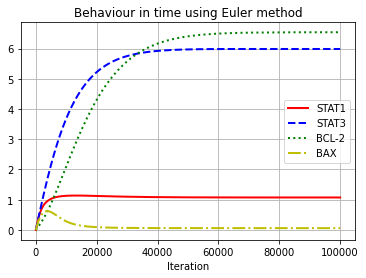
\includegraphics[width=0.6\textwidth]{Figures/A.JPG}
% 	\end{framed}
% 	\caption{Two blocks are attached to three springs \cite{Departme83:online}.}
% 	\label{fig:1}
% \end{figure}


\subsection{Mathematical modelling for cell signalling}

The term "biological system" can be interpreted in a variety of ways at different organisational levels, necessitating unique approaches and methodologies for modelling and analysis. Metabolic systems, cell cycle regulation, development and differentiation, as well as intra- and intercellular signalling and cell communication, are all included. The majority of the related underlying processes exhibit dynamic activity. Changes in gene expression patterns or metabolite profiles, as well as fluctuations in protein and hormone levels, are examples of this, particularly in response to altered environmental conditions or pharmacological modulation \cite{feitelson2015sustained}. Cellular signalling is a component of complex system communication, directing basic as well as cell-type specific cellular functions and coordinating cell actions in unicellular and multicellular organisms \cite{danos2007rule}. Beginning with the activation of a cell surface receptor, intracellular signalling molecules are then changed, allowing the evoked initial signal to be transmitted to the targeted cell response. These signalling events do not always go in a straight line, relaying and regulating information from cell surface receptors to effectors like transcription factors or specific enzymes. Cellular signalling networks are made up of highly coupled modules that regulate many processes in context, including regulatory feedback \cite{jordan2000interleukin}.

\section{Problem statement and objectives}
\paragraph{}

Apoptosis is a crucial biological process that regulates cell death in response to various stimuli. It is a complex process that involves several key signaling pathways and intercellular modules. The Intercellular modules such as STAT1, STAT3, Bcl-2 and BAX play a critical role in apoptosis signaling. Understanding the dynamics of these modules and how they interact with each other is crucial for gaining insights into the apoptosis process.

This project aims to conduct numerical investigations of the Intercellular modules (STAT1, STAT3, Bcl-2, and BAX) involved in apoptosis signalling. The project will focus on two methods for numerical investigations, namely Euler's method and the Runge-Kutta fourth-order method. The main focus of this project is to understand the behavior of these modules in response to the activation of the IFN-$\beta$ and JAK2 signalling pathways.

Euler's method is a basic numerical method used to solve ordinary differential equations (ODEs). It is a simple method that uses a straight-line approximation to estimate the solution to an ODE. However, Euler's method is not very accurate and can be prone to error, especially when the solution changes rapidly. Despite this, it is still widely used as a first step in solving ODEs, as it provides a simple and straightforward approach to solving ODEs.

The Runge-Kutta fourth-order method is a more sophisticated numerical method that provides improved accuracy compared to Euler's method. It uses a combination of multiple straight-line approximations to estimate the solution to an ODE. This method is considered more accurate and efficient compared to Euler's method and is commonly used to solve complex ODEs.

The numerical investigations will be conducted by representing the levels of the Intercellular modules (STAT1, STAT3, Bcl-2, and BAX) and their activity by mathematical variables. The behaviour of the modules will be analyzed and compared using both Euler's method and the Runge-Kutta fourth-order method. The results of the numerical investigations will be visualized and compared, allowing for a better understanding of the behaviour of the Intercellular modules in response to the activation of the IFN-$\beta$ and JAK2 signalling pathways.

The mathematical equilibrium and stability analysis will involve finding the steady-state solutions and determining their stability for the systems representing the Intercellular modules and their interactions. The equilibrium and stability analysis results will provide essential insights into the long-term behaviour of the modules.

In conclusion, this project aims to provide a deeper understanding of the behaviour of Intercellular modules (STAT1, STAT3, Bcl-2, and BAX) involved in apoptosis signalling by combining the mathematical equilibrium and stability analysis and numerical investigations. The numerical investigations using Euler's method and the Runge-Kutta fourth-order method will provide valuable insights into the dynamics of these modules and their interactions with each other. This project is expected to contribute to the field of apoptosis research and provide a foundation for further studies on the apoptosis signalling network.



\section{Project structure}
\paragraph{}

This project focuses on mathematical modeling approaches for cell signalling and aims to understand the genetic alterations in signalling pathways in cancer and their downstream signalling. The project starts with a background of the study where mathematical modelling approaches and their application for cell signalling are introduced. The problem statement and objectives are then highlighted. The project structure is outlined, which includes the theoretical background, methodology, numerical method for ordinary differential equations, results and discussion, and conclusion.

The theoretical background covers a biological introduction of cell signalling and explains genetic alterations in signalling pathways and their relevance to cancer. It provides an in-depth look at receptor tyrosine kinases in cancer and their downstream signalling, along with a summary of the current state of knowledge about the signalling pathways involved in cancer and the challenges in understanding these pathways. Numerical analysis is also briefly mentioned.

The methodology section of the project explains the biological approach of STAT1, STAT3, Bcl-2 and BAX and then moves on to a mathematical model for the intracellular module of these proteins. The mathematical model includes a schematic diagram of the apoptosis signalling network and the governing ordinary differential equations for the intracellular signalling network. The section concludes with mathematical equilibrium and stability analysis.

The numerical method for ordinary differential equations section explains the numerical investigation using Euler’s method, the numerical integration technique for the Runge-Kutta fourth-order method, and other relevant details. The results and discussion section present the numerical results for different scenarios, such as S=0 and J=0, S=0 and J=1, S=0.4 and J=0, and S=1 and J=1. The section concludes with an equilibrium and stability analysis.

The project concludes with a summary of the findings and recommendations for future research.  
\paragraph{}







































 

 
 
\chapter{Introduction}
\label{chap:01}


\paragraph{}


 Models in cell biology are both familiar and mysterious. On the one hand, biologists have traditionally utilised models to represent reality, such as diagrams, rules, graphs, plots, chemical formulas, and relationships. Their purpose is to be similar to numerous organisms while not being the same. As a result, it is reasonable to suppose that discoveries will also shed light on the workings of other organisms. On the other hand, a mathematical representation of biological systems and processes can be understood as a model, forming a relatively recent branch of biological study. A mathematical model, according to Eykhoff \cite{serra2011using}, is "a representation of the main elements of an existing system (or a system to be developed) that offers knowledge of that system in useable form." Mathematical models can take numerous forms and are especially effective for data-integrative studies of interactions between different components of biological systems and the way these interactions affect the overall function and behaviour of a system \cite{kapur1988mathematical}. This processes biological modelling approach connects fundamental chemical and physical principles, prior knowledge of the researched system, and experimental data to create a robust tool for extending and formalising classical cell biology \cite{motta2013mathematical,friedman2014mathematical}. Unscrambling an organism's genome is undoubtedly a first step toward understanding mechanisms in living cells; nevertheless, a complete image is required to truly capture the regulatory features of genetic, metabolic, and cellular signalling networks \cite{gold1977mathematical}. This is supported by mathematical formulation, hypothesis creation, and comparison validation with experimental data \cite{almeida2021formulation}. Data-driven calibrated models have the ability to generate new hypotheses and predictions, and they represent a guided approach to building promising continuous experiments to investigate issues that are not susceptible to experimental investigation. Simultaneously, experiment results are frequently too complicated to be understood by visual examination and can be related.
 


\section{Background of the study}
\label{sec:1.1}

\paragraph{}

The study of linked mathematical modeling has since become an essential branch of mathematics, with applications in physics, biology, and chemistry \cite{fowler1997mathematical}. A simulation is a mathematical depiction of a physical, biological, or information system.  Models enable us to think about a system and forecast its behaviour. A dynamical system is one in which the consequences of actions do not arise instantly.  For example, a headache does not go away immediately after taking aspirin; it takes time to take action. Additional funding for a development project does not enhance profits in the  short term, but it may do the same in the longer - term in enterprise applications. These are dynamic systems instances in which the system's behaviour varies over time. Most species directly correspond to numerous patterns in our environment, such as the earth's rotation around the sun, the alternation of night and day, or the tides. But in this project, mathematical modeling for cancer signalling will be discussed. 


\subsection{Mathematical modeling approaches}
\paragraph{}

There are many different approaches to mathematical modeling that can be used in the study of cancer. The choice of approach will depend on the specific research question being addressed and the characteristics of the cancerous system being studied. Some common approaches to mathematical modeling in cancer research include:

\begin{itemize}
    \item Deterministic models: These models can be used to describe the relationships between different signalling pathways and the behaviour of cancer cells and to predict the effects of different perturbations on the system \cite{altrock2015mathematics}, such as mutations or the inhibition of specific signalling proteins \cite{tabassum2019mathematical}.

    \item Stochastic models: These models can be used to describe the randomness or uncertainty inherent in cancerous systems and can be used to study how random events, such as gene mutations, contribute to the development and progression of cancer \cite{tsodikov1996stochastic}.

    \item Agent-based models: These models can be used to represent the behaviour of individual cancer cells or the interactions between cancer cells and the surrounding tissue and can be used to study how the collective behaviour of cancer cells emerges from their individual behaviour \cite{figueredo2013investigating}.

    \item Network models: These models can be used to represent the interactions between different signalling pathways and molecules in cancerous systems and can be used to study how these interactions contribute to the development and progression of cancer \cite{ji2020mathematical}.

    \item Dynamical systems models: These models can be used to describe the evolution of cancerous systems over time and can be used to study how cancer cells adapt and respond to different stimuli or perturbations \cite{haupt2021mathematical}.
\end{itemize}

Again, these are just a few examples, and researchers may use a combination of different approaches to best capture the behaviour of a particular cancerous system. All strategies include assumptions about the system under consideration, necessitate specific sorts of measurements, and allow for conclusions with varying degrees of accuracy and detail.





%  \begin{figure}[hbt!]
% 	\centering
% 	\begin{framed}
% 	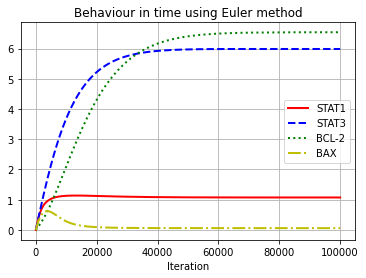
\includegraphics[width=0.6\textwidth]{Figures/A.JPG}
% 	\end{framed}
% 	\caption{Two blocks are attached to three springs \cite{Departme83:online}.}
% 	\label{fig:1}
% \end{figure}


\subsection{Mathematical modelling for cell signalling}

The term "biological system" can be interpreted in a variety of ways at different organisational levels, necessitating unique approaches and methodologies for modelling and analysis. Metabolic systems, cell cycle regulation, development and differentiation, as well as intra- and intercellular signalling and cell communication, are all included. The majority of the related underlying processes exhibit dynamic activity. Changes in gene expression patterns or metabolite profiles, as well as fluctuations in protein and hormone levels, are examples of this, particularly in response to altered environmental conditions or pharmacological modulation \cite{feitelson2015sustained}. Cellular signalling is a component of complex system communication, directing basic as well as cell-type specific cellular functions and coordinating cell actions in unicellular and multicellular organisms \cite{danos2007rule}. Beginning with the activation of a cell surface receptor, intracellular signalling molecules are then changed, allowing the evoked initial signal to be transmitted to the targeted cell response. These signalling events do not always go in a straight line, relaying and regulating information from cell surface receptors to effectors like transcription factors or specific enzymes. Cellular signalling networks are made up of highly coupled modules that regulate many processes in context, including regulatory feedback \cite{jordan2000interleukin}.

\section{Problem statement and objectives}
\paragraph{}

Apoptosis is a crucial biological process that regulates cell death in response to various stimuli. It is a complex process that involves several key signaling pathways and intercellular modules. The Intercellular modules such as STAT1, STAT3, Bcl-2 and BAX play a critical role in apoptosis signaling. Understanding the dynamics of these modules and how they interact with each other is crucial for gaining insights into the apoptosis process.

This project aims to conduct numerical investigations of the Intercellular modules (STAT1, STAT3, Bcl-2, and BAX) involved in apoptosis signalling. The project will focus on two methods for numerical investigations, namely Euler's method and the Runge-Kutta fourth-order method. The main focus of this project is to understand the behavior of these modules in response to the activation of the IFN-$\beta$ and JAK2 signalling pathways.

Euler's method is a basic numerical method used to solve ordinary differential equations (ODEs). It is a simple method that uses a straight-line approximation to estimate the solution to an ODE. However, Euler's method is not very accurate and can be prone to error, especially when the solution changes rapidly. Despite this, it is still widely used as a first step in solving ODEs, as it provides a simple and straightforward approach to solving ODEs.

The Runge-Kutta fourth-order method is a more sophisticated numerical method that provides improved accuracy compared to Euler's method. It uses a combination of multiple straight-line approximations to estimate the solution to an ODE. This method is considered more accurate and efficient compared to Euler's method and is commonly used to solve complex ODEs.

The numerical investigations will be conducted by representing the levels of the Intercellular modules (STAT1, STAT3, Bcl-2, and BAX) and their activity by mathematical variables. The behaviour of the modules will be analyzed and compared using both Euler's method and the Runge-Kutta fourth-order method. The results of the numerical investigations will be visualized and compared, allowing for a better understanding of the behaviour of the Intercellular modules in response to the activation of the IFN-$\beta$ and JAK2 signalling pathways.

The mathematical equilibrium and stability analysis will involve finding the steady-state solutions and determining their stability for the systems representing the Intercellular modules and their interactions. The equilibrium and stability analysis results will provide essential insights into the long-term behaviour of the modules.

In conclusion, this project aims to provide a deeper understanding of the behaviour of Intercellular modules (STAT1, STAT3, Bcl-2, and BAX) involved in apoptosis signalling by combining the mathematical equilibrium and stability analysis and numerical investigations. The numerical investigations using Euler's method and the Runge-Kutta fourth-order method will provide valuable insights into the dynamics of these modules and their interactions with each other. This project is expected to contribute to the field of apoptosis research and provide a foundation for further studies on the apoptosis signalling network.



\section{Project structure}
\paragraph{}

This project focuses on mathematical modeling approaches for cell signalling and aims to understand the genetic alterations in signalling pathways in cancer and their downstream signalling. The project starts with a background of the study where mathematical modelling approaches and their application for cell signalling are introduced. The problem statement and objectives are then highlighted. The project structure is outlined, which includes the theoretical background, methodology, numerical method for ordinary differential equations, results and discussion, and conclusion.

The theoretical background covers a biological introduction of cell signalling and explains genetic alterations in signalling pathways and their relevance to cancer. It provides an in-depth look at receptor tyrosine kinases in cancer and their downstream signalling, along with a summary of the current state of knowledge about the signalling pathways involved in cancer and the challenges in understanding these pathways. Numerical analysis is also briefly mentioned.

The methodology section of the project explains the biological approach of STAT1, STAT3, Bcl-2 and BAX and then moves on to a mathematical model for the intracellular module of these proteins. The mathematical model includes a schematic diagram of the apoptosis signalling network and the governing ordinary differential equations for the intracellular signalling network. The section concludes with mathematical equilibrium and stability analysis.

The numerical method for ordinary differential equations section explains the numerical investigation using Euler’s method, the numerical integration technique for the Runge-Kutta fourth-order method, and other relevant details. The results and discussion section present the numerical results for different scenarios, such as S=0 and J=0, S=0 and J=1, S=0.4 and J=0, and S=1 and J=1. The section concludes with an equilibrium and stability analysis.

The project concludes with a summary of the findings and recommendations for future research.  
\paragraph{}







































%\chapter{Introduction}
\label{chap:01}


\paragraph{}


 Models in cell biology are both familiar and mysterious. On the one hand, biologists have traditionally utilised models to represent reality, such as diagrams, rules, graphs, plots, chemical formulas, and relationships. Their purpose is to be similar to numerous organisms while not being the same. As a result, it is reasonable to suppose that discoveries will also shed light on the workings of other organisms. On the other hand, a mathematical representation of biological systems and processes can be understood as a model, forming a relatively recent branch of biological study. A mathematical model, according to Eykhoff \cite{serra2011using}, is "a representation of the main elements of an existing system (or a system to be developed) that offers knowledge of that system in useable form." Mathematical models can take numerous forms and are especially effective for data-integrative studies of interactions between different components of biological systems and the way these interactions affect the overall function and behaviour of a system \cite{kapur1988mathematical}. This processes biological modelling approach connects fundamental chemical and physical principles, prior knowledge of the researched system, and experimental data to create a robust tool for extending and formalising classical cell biology \cite{motta2013mathematical,friedman2014mathematical}. Unscrambling an organism's genome is undoubtedly a first step toward understanding mechanisms in living cells; nevertheless, a complete image is required to truly capture the regulatory features of genetic, metabolic, and cellular signalling networks \cite{gold1977mathematical}. This is supported by mathematical formulation, hypothesis creation, and comparison validation with experimental data \cite{almeida2021formulation}. Data-driven calibrated models have the ability to generate new hypotheses and predictions, and they represent a guided approach to building promising continuous experiments to investigate issues that are not susceptible to experimental investigation. Simultaneously, experiment results are frequently too complicated to be understood by visual examination and can be related.
 


\section{Background of the study}
\label{sec:1.1}

\paragraph{}

The study of linked mathematical modeling has since become an essential branch of mathematics, with applications in physics, biology, and chemistry \cite{fowler1997mathematical}. A simulation is a mathematical depiction of a physical, biological, or information system.  Models enable us to think about a system and forecast its behaviour. A dynamical system is one in which the consequences of actions do not arise instantly.  For example, a headache does not go away immediately after taking aspirin; it takes time to take action. Additional funding for a development project does not enhance profits in the  short term, but it may do the same in the longer - term in enterprise applications. These are dynamic systems instances in which the system's behaviour varies over time. Most species directly correspond to numerous patterns in our environment, such as the earth's rotation around the sun, the alternation of night and day, or the tides. But in this project, mathematical modeling for cancer signalling will be discussed. 


\subsection{Mathematical modeling approaches}
\paragraph{}

There are many different approaches to mathematical modeling that can be used in the study of cancer. The choice of approach will depend on the specific research question being addressed and the characteristics of the cancerous system being studied. Some common approaches to mathematical modeling in cancer research include:

\begin{itemize}
    \item Deterministic models: These models can be used to describe the relationships between different signalling pathways and the behaviour of cancer cells and to predict the effects of different perturbations on the system \cite{altrock2015mathematics}, such as mutations or the inhibition of specific signalling proteins \cite{tabassum2019mathematical}.

    \item Stochastic models: These models can be used to describe the randomness or uncertainty inherent in cancerous systems and can be used to study how random events, such as gene mutations, contribute to the development and progression of cancer \cite{tsodikov1996stochastic}.

    \item Agent-based models: These models can be used to represent the behaviour of individual cancer cells or the interactions between cancer cells and the surrounding tissue and can be used to study how the collective behaviour of cancer cells emerges from their individual behaviour \cite{figueredo2013investigating}.

    \item Network models: These models can be used to represent the interactions between different signalling pathways and molecules in cancerous systems and can be used to study how these interactions contribute to the development and progression of cancer \cite{ji2020mathematical}.

    \item Dynamical systems models: These models can be used to describe the evolution of cancerous systems over time and can be used to study how cancer cells adapt and respond to different stimuli or perturbations \cite{haupt2021mathematical}.
\end{itemize}

Again, these are just a few examples, and researchers may use a combination of different approaches to best capture the behaviour of a particular cancerous system. All strategies include assumptions about the system under consideration, necessitate specific sorts of measurements, and allow for conclusions with varying degrees of accuracy and detail.





%  \begin{figure}[hbt!]
% 	\centering
% 	\begin{framed}
% 	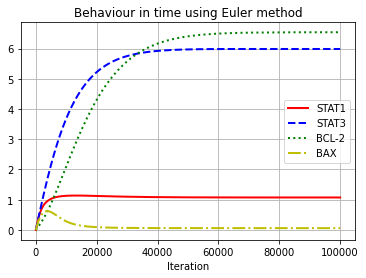
\includegraphics[width=0.6\textwidth]{Figures/A.JPG}
% 	\end{framed}
% 	\caption{Two blocks are attached to three springs \cite{Departme83:online}.}
% 	\label{fig:1}
% \end{figure}


\subsection{Mathematical modelling for cell signalling}

The term "biological system" can be interpreted in a variety of ways at different organisational levels, necessitating unique approaches and methodologies for modelling and analysis. Metabolic systems, cell cycle regulation, development and differentiation, as well as intra- and intercellular signalling and cell communication, are all included. The majority of the related underlying processes exhibit dynamic activity. Changes in gene expression patterns or metabolite profiles, as well as fluctuations in protein and hormone levels, are examples of this, particularly in response to altered environmental conditions or pharmacological modulation \cite{feitelson2015sustained}. Cellular signalling is a component of complex system communication, directing basic as well as cell-type specific cellular functions and coordinating cell actions in unicellular and multicellular organisms \cite{danos2007rule}. Beginning with the activation of a cell surface receptor, intracellular signalling molecules are then changed, allowing the evoked initial signal to be transmitted to the targeted cell response. These signalling events do not always go in a straight line, relaying and regulating information from cell surface receptors to effectors like transcription factors or specific enzymes. Cellular signalling networks are made up of highly coupled modules that regulate many processes in context, including regulatory feedback \cite{jordan2000interleukin}.

\section{Problem statement and objectives}
\paragraph{}

Apoptosis is a crucial biological process that regulates cell death in response to various stimuli. It is a complex process that involves several key signaling pathways and intercellular modules. The Intercellular modules such as STAT1, STAT3, Bcl-2 and BAX play a critical role in apoptosis signaling. Understanding the dynamics of these modules and how they interact with each other is crucial for gaining insights into the apoptosis process.

This project aims to conduct numerical investigations of the Intercellular modules (STAT1, STAT3, Bcl-2, and BAX) involved in apoptosis signalling. The project will focus on two methods for numerical investigations, namely Euler's method and the Runge-Kutta fourth-order method. The main focus of this project is to understand the behavior of these modules in response to the activation of the IFN-$\beta$ and JAK2 signalling pathways.

Euler's method is a basic numerical method used to solve ordinary differential equations (ODEs). It is a simple method that uses a straight-line approximation to estimate the solution to an ODE. However, Euler's method is not very accurate and can be prone to error, especially when the solution changes rapidly. Despite this, it is still widely used as a first step in solving ODEs, as it provides a simple and straightforward approach to solving ODEs.

The Runge-Kutta fourth-order method is a more sophisticated numerical method that provides improved accuracy compared to Euler's method. It uses a combination of multiple straight-line approximations to estimate the solution to an ODE. This method is considered more accurate and efficient compared to Euler's method and is commonly used to solve complex ODEs.

The numerical investigations will be conducted by representing the levels of the Intercellular modules (STAT1, STAT3, Bcl-2, and BAX) and their activity by mathematical variables. The behaviour of the modules will be analyzed and compared using both Euler's method and the Runge-Kutta fourth-order method. The results of the numerical investigations will be visualized and compared, allowing for a better understanding of the behaviour of the Intercellular modules in response to the activation of the IFN-$\beta$ and JAK2 signalling pathways.

The mathematical equilibrium and stability analysis will involve finding the steady-state solutions and determining their stability for the systems representing the Intercellular modules and their interactions. The equilibrium and stability analysis results will provide essential insights into the long-term behaviour of the modules.

In conclusion, this project aims to provide a deeper understanding of the behaviour of Intercellular modules (STAT1, STAT3, Bcl-2, and BAX) involved in apoptosis signalling by combining the mathematical equilibrium and stability analysis and numerical investigations. The numerical investigations using Euler's method and the Runge-Kutta fourth-order method will provide valuable insights into the dynamics of these modules and their interactions with each other. This project is expected to contribute to the field of apoptosis research and provide a foundation for further studies on the apoptosis signalling network.



\section{Project structure}
\paragraph{}

This project focuses on mathematical modeling approaches for cell signalling and aims to understand the genetic alterations in signalling pathways in cancer and their downstream signalling. The project starts with a background of the study where mathematical modelling approaches and their application for cell signalling are introduced. The problem statement and objectives are then highlighted. The project structure is outlined, which includes the theoretical background, methodology, numerical method for ordinary differential equations, results and discussion, and conclusion.

The theoretical background covers a biological introduction of cell signalling and explains genetic alterations in signalling pathways and their relevance to cancer. It provides an in-depth look at receptor tyrosine kinases in cancer and their downstream signalling, along with a summary of the current state of knowledge about the signalling pathways involved in cancer and the challenges in understanding these pathways. Numerical analysis is also briefly mentioned.

The methodology section of the project explains the biological approach of STAT1, STAT3, Bcl-2 and BAX and then moves on to a mathematical model for the intracellular module of these proteins. The mathematical model includes a schematic diagram of the apoptosis signalling network and the governing ordinary differential equations for the intracellular signalling network. The section concludes with mathematical equilibrium and stability analysis.

The numerical method for ordinary differential equations section explains the numerical investigation using Euler’s method, the numerical integration technique for the Runge-Kutta fourth-order method, and other relevant details. The results and discussion section present the numerical results for different scenarios, such as S=0 and J=0, S=0 and J=1, S=0.4 and J=0, and S=1 and J=1. The section concludes with an equilibrium and stability analysis.

The project concludes with a summary of the findings and recommendations for future research.  
\paragraph{}







































\chapter{Theoretical Background}
\label{chap:02}
\paragraph{}
Cell-cell signalling is the process by which cells communicate with each other within the body. This communication can occur between cells that are next-door neighbours or between cells that are far apart. There are several different types of cell-cell signalling, including paracrine signalling, autocrine signalling, endocrine signalling, and synaptic signalling. In terms of numerical methods, these are mathematical techniques that are used to model and simulate complex systems. Numerical methods can be used to study a wide range of problems, including those in physics, engineering, and biology. In the context of cell-cell signalling, numerical methods can be used to model the dynamics of signalling pathways, predict the behaviour of cells in response to different signals, and design new drugs that target specific signalling pathways. These methods can include techniques such as differential equations, linear algebra, and optimization. So in this chapter theoretical background of cancer cell-cell signalling and its mathematical background will be discussed. 

\subsection{Biological introduction of cell signalling}
\paragraph{}
Cells develop and proliferate out of control in cancer, which is a disease. Cancer cells create a number of distinctive modifications in their cell signalling pathways as the tumour grows \cite{peng2017lncrna}. These modifications include the ability to proliferate without exogenous growth-promoting or growth-inhibitory signals, invade nearby tissues and metastasize to distant sites, elicit an angiogenic response, and evade cell proliferation-limiting mechanisms like apoptosis and senescence \cite{crosas2022rho}. Understanding these changes in cell signalling pathways and how they affect the onset and spread of cancer is the primary goal of research in cancer biology and cell signalling. For the purpose of enhancing precision medicine treatments for hormone-related and genitourinary cancers, this includes researching tumour evolution, drug sensitization, and oncogene network modifications in patients. 

Cytokine receptors and receptor tyrosine kinases (RTKs) are proteins that start cell signalling cascades \cite{kazi2014socs}. The intracellular section of RTKs has a tyrosine kinase domain that enables them to phosphorylate other proteins, initiating a signalling cascade. On the other hand, in order to start signalling, cytokine receptors need to join forces with other intracellular proteins known as Janus kinases (JAKs) \cite{gadina2013janus}. A cytokine receptor that is not linked to a JAK molecule lacks the kinase activity that the JAK molecules have. Both varieties of receptors start the intracellular signalling pathways when they attach to particular substances in the extracellular environment known as ligands. The sort of ligands that these two types of receptors bind—RTKs mainly bind to growth factors, whereas Cytokine receptors primarily bind to cytokines—is the fundamental distinction between them \cite{tamiya2011suppressors}.

 \begin{figure}[hbt!]
	\centering
	\begin{framed}
	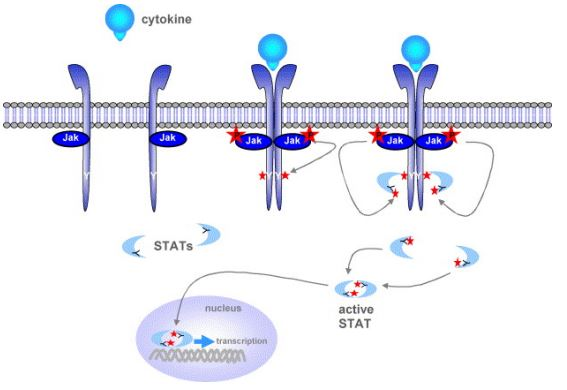
\includegraphics[width=0.8\textwidth]{Figures/a.JPG}
		\end{framed}
	\caption{Diagram of the JAK/STAT signalling pathway, initiated by cytokine molecules, taken from \cite{haan2006jaks}. The red stars attached to a species indicate that the species is phosphorylated.}
	\label{fig:6}
\end{figure}

\subsection{Genetic alterations in signalling pathways}
\paragraph{}

Modifications in the genes that regulate cellular processes like cell division and cell death are referred to as genetic changes in signalling pathways\cite{strasser2000apoptosis}. These changes can be brought about by gene fusions, copy-number changes, mutations, and mRNA expression \cite{kang2016integrated}. These modifications can result in the unchecked cell growth and proliferation that characterise cancer. Melanoma, where mutations in the RAS signalling cascade are almost universally present, is one example of genetic changes in signalling pathways. Although RAS itself is rarely mutated in melanoma, RAS is downstream from BRAF on the protein kinase B/Akt pathway and PTEN on the mitogen-activated protein kinase pathway. These genes are frequently altered in melanomas; BRAF is the most frequently mutated gene in melanomas \cite{haluska2006genetic}. Understanding the genetic alterations in signaling pathways is an essential aspect of cancer research and treatment, as these alterations can be targeted with drugs and therapies to limit the growth and spread of cancer cells. 



\subsection{RORs (Receptor Tyrosine Kinases) in cancer and its downstream signalling}
\paragraph{}

Receptor Tyrosine Kinases (RTKs) play a critical role in cancer by initiating cell signalling pathways \cite{butti2018receptor}. RORs (Receptors of RAS-related Orphans) are a subfamily of RTKs that have been shown to impact cancer significantly \cite{kamrani2019therapeutic}. RORs are a group of receptors that are activated by ligands and are involved in cell growth, differentiation and the formation of blood vessels. In cancer, RORs are often dysregulated, and this leads to overactive or abnormal signalling within and among these pathways that may contribute to the survival of cancer stem cells (CSCs). The dysregulation of RORs can lead to the formation of new blood vessels, the ability of cancer cells to migrate and invade other tissues, and the resistance to chemotherapy and radiation therapy \cite{pan2016emerging, mahmoudian2021interaction}. To understand it better, refer to Figure \ref{fig:2}, which will help you understand the process more precisely and engagingly. This image will provide a visual representation of how RORs work in cancer and how they contribute to the development of cancer. Additionally, it will also provide a better understanding of the downstream signalling pathways that are activated by RORs and how they lead to the formation of cancer.


 \begin{figure}[hbt!]
	\centering
	\begin{framed}
	\includegraphics[width=0.8\textwidth]{Figures/b.png}
		\end{framed}
	\caption{ROR1 signaling. WNT/ROR1 signalling is induced by the binding of a non-canonical WNT ligand, which triggers the formation of a complex between ROR1 and ROR2, or ROR1 and a FZD receptor, respectively \cite{menck2021wnt}. }
	\label{fig:2}
\end{figure}

\subsection{The current state of knowledge about the signalling pathways involved in cancer and the challenges in understanding these pathways.}
\paragraph{}

The aberrant cell proliferation that characterises cancer is a complex disease. Numerous signalling pathways have been linked to the development and spread of cancer, but the precise processes by which these pathways cause the disease are still poorly understood. The RAS signalling cascade, which is frequently changed in a range of tumour forms, is one of the important signalling pathways in cancer \cite{maruta1994regulation}. A mutation in a member of the RAS family of proteins, which is involved in cell growth and differentiation, can result in uncontrolled cell proliferation and the emergence of cancer. Other signalling pathways like PI3K-Akt, Wnt, and Notch have also been discovered to have a role in the development and spread of cancer \cite{rizzatti2005gene, lombardi2013solar}.

The complexity of the interactions between many signalling channels presents one of the difficulties in understanding these pathways. It is challenging to pinpoint the precise function of any one process in the disease, for instance, because alterations in one pathway can affect the activity of other pathways. The fact that numerous alternative pathways can activate the same pathway further complicates our knowledge of the disease. Cancer is a diverse illness, and various cancer forms might have various genetic and molecular alterations. Consequently, it is challenging to create targeted medicines that are efficient in treating all cancer types \cite{meng2017identification, hansen2015gut}. 

In conclusion, there is still much to learn about the precise methods by which the signalling pathways involved in cancer contribute to the disease. These pathways are intricate and multifaceted. Further study is required to comprehend these pathways better and create cancer medicines that work.

\subsection{Numerical analysis}
\label{Num}

\paragraph{}
Numerical analysis is a branch of mathematics that teaches computer methods for studying and solving mathematical issues \cite{burden2015numerical}. In this section, we look at numerical approaches for solving the most frequent mathematical problems and analyse the errors that can occur while using these methods. Because practically all computation is now done on digital computers, we also explore the consequences of numerical method implementation.

The investigation of errors is vital to numerical analysis. Most numerical approaches produce responses that are simply approximations of the intended genuine solution, and it is critical to understand the associated error and, if feasible, estimate or constrain it \cite{heydari2016theoretical}. This study looks at the numerous errors that can occur in a situation. The representation of numbers in computers, as well as the mistake in computer arithmetic, are investigated \cite{cui2018numerical}. The general results on the propagation of errors in calculations are presented, along with a detailed examination of errors in summing processes. Especially in this study, we will consider the Runge Kutta fourth-order (RK4) method \cite{islam2015comparative}. 

\subsubsection{Runge Kutta fourth order method}
\label{RK}

\paragraph{}

The fourth-order Runge-Kutta technique explains the lengthy computation of numerous unknowns, and the comprehensive step-by-step derivation and analysis can be found in many publications \cite{tan2012general, mehdi2017using}. Because of the method's importance in mathematics and applied science/engineering. By reviewing specific, possibly well-known papers, we simplify and minimise the complexity of their derivation and analysis by proposing a step-by-step derivation of the method.

In 1901, two German men, Carl Runge (1856-1927) and Martin Kutta (1867-1944), devised the Runge-Kutta Method \cite{tobies2012iris}. Carl Runge created numerical methods for solving differential equations that evolved from his research on atomic spectra. These numerical techniques are still in use today. He employed so much mathematics in his studies that physicists mistook him for a mathematician, and he employed so much physics that mathematicians mistook him for a physicist. His name is now synonymous with the Runge-Kutta methods for numerically solving differential equations. Kutta, another German applied mathematician, is well recognised for his contribution to the Kutta-Joukowski theory of airfoil lift in aerodynamics, which is based on differential equations \cite{trefethen2015invented}. 


\subsubsection{Runge-Kutta 4th order method to solve differential equation}

Given the following inputs \cite{rungekutta_2023_webpage}. 

\begin{itemize}
    \item An ordinary differential equation that expresses the value of $dy/dt$ in terms of $t$ and $y$.
    \item Initial value of $y$, i.e., $y(0)$. 
\end{itemize}

\begin{equation}
    {{dy(t)} \over {dt}} = y'(t) = f(y(t),t), \quad \quad {\rm{with\;}} y(t_0)=y_0
\end{equation}

The evolution of the Fourth Order Runge-Kutta method closely parallels that of the second Order and will not be discussed in depth here. Like the second-order method, the fourth-order method has several variations that all employ four estimates of the slope. To determine the slope at some time t0 (assuming we just have an approximation to $y(t_0)$ (which we call $y^*(t_0)$), we will utilise the following slope approximations.

 \begin{figure}[hbt!]
	\centering
	\begin{framed}
	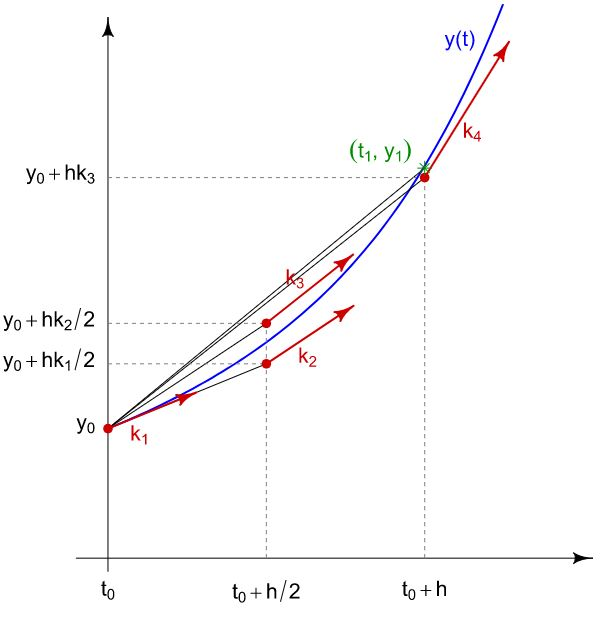
\includegraphics[width=0.7\textwidth]{Figures/F.JPG}
		\end{framed}
	\caption{Slopes used by the classical Runge-Kutta method \cite{hossain2017comparative}.}
	\label{fig:6}
\end{figure}

\newpage

\begin{equation}
    {k_1} = f({y^*}({t_0}),{t_0})
\end{equation}

\begin{equation}
    {k_2} = f\left( {{y^*}({t_0}) + {k_1}{h \over 2},{t_0} + {h \over 2}} \right)
\end{equation}

\begin{equation}
     {k_3} = f\left( {{y^*}({t_0}) + {k_2}{h \over 2},{t_0} + {h \over 2}} \right) 
\end{equation}

\begin{equation}
    {k_4} = f\left( {{y^*}({t_0}) + {k_3}h,{t_0} + h} \right)
\end{equation}

Each one of these slope estimates can be directly explained. 

\begin{itemize}
    \item $k_1$ is the slope at the beginning of the time step (this is the same as $k_1$ in the first and second order methods).
    
\item If we use the slope $k_1$ to step halfway through the time step, then $k_2$ is an estimate of the slope at the midpoint. This is the same as the slope $k_2$, from the second-order midpoint method. This slope proved to be more accurate than $k_1$ for making new approximations for y(t).

\item If we use the slope $k_2$ to step halfway through the time step, then $k_3$ is another estimate of the slope at the midpoint.

\item Finally, we use the slope, $k_3$, to step all the way across the time step$(t_0, t_0+h)$, and $k_4$ is an estimate of the slope at the endpoint. 
\end{itemize}

We then use a weighted sum of these slopes to get our final estimate of $y^*(t_0+h)$.

\begin{equation}
    {y^*}({t_0} + h) = {y^*}({t_0}) + {{{k_1} + 2{k_2} + 2{k_3} + {k_4}} \over 6}h 
\end{equation}



\begin{equation}
   {y^*}({t_0} + h) = {y^*}({t_0}) + \left( {{1 \over 6}{k_1} + {1 \over 3}{k_2} + {1 \over 3}{k_3} + {1 \over 6}{k_4}} \right)h
\end{equation}

\begin{equation}
   {y^*}({t_0} + h) =  {y^*}({t_0}) + mh
\end{equation}

 {\rm{where\;}}m{\rm{\;is\;a\;weighted\;average\; slope\; approximation.}}

The approach is comparable to the second-order endpoint method \cite{dontchev2000second}, which employed an equal weighting of the slopes at the start and end of the interval. The weighting of the midpoint slopes ($k_2$ and $k_3$) is larger than that of the endpoint slopes ($k_1$ and $k_4$) in this case because we expect these to be a better estimate of the slope while travelling from $y^*(t_0)$ to $y^*(t_0+h)$.

\newpage
 \subsubsection{Euler's numerical method}
 \paragraph{}

Euler's method is a numerical method used to approximate solutions to first-order ordinary differential equations (ODEs) called initial value problems. It is named after the Swiss mathematician Leonhard Paul Euler (1707-1783) \cite{biswas2013discussion, zondervan1998review}. The basic idea behind Euler's method is to approximate the solution of an ODE by constructing tangents to the solution curve at discrete points using a simple formula. The method is based on the assumption that the tangent line to the solution curve of the ODE at a given point approximates the solution curve over a small interval. Euler's method uses the simple formula, $y(x+h) = y(x) + hf(x,y)$ to construct the tangent at the point x and obtain the value of y(x+h), whose slope is $f(x,y)$ \cite{mazandarani2013modified}. This method can be used to approximate the solution of a first-order ODE by creating a sequence of short-line segments at steps of $h$. However, Euler's method is considered crude and not widely used in practice due to its low accuracy. 

\subsubsection{Euler's method to solve differential equation}
\paragraph{}

Euler's method is a first-order numerical procedure for solving ordinary differential equations (ODEs) with a given initial value. 

 \begin{figure}[hbt!]
	\centering
	\begin{framed}
	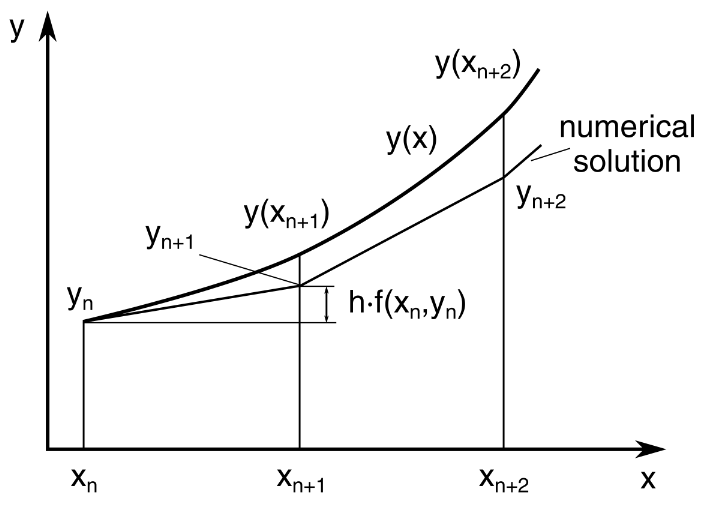
\includegraphics[width=0.65\textwidth]{Figures/euler.PNG}
		\end{framed}
	\caption{Slopes used by the Euler's method \cite{freecodecamp.org_2021}.}
	\label{fig:6}
\end{figure}


The general initial value problem methodology is given by the equation: 

\begin{equation}
    x_n = x_0 + nh
\end{equation}
\begin{equation}
    y_n = y_{n-1} + hf(x_{n-1}, y_{n-1})
\end{equation}

where $h$ represents the step size and $n$ is an integer, starting with 1. The number of steps taken is counted by the variable $n$. This method is based on the assumption that the tangent line to the integral curve of the ODE at $(x_n, y(x_n))$ approximates the integral curve over the interval $[x_n, x_{n + 1}]$. The formula used in Euler's method is:

\begin{equation}
    y(x+h) = y(x) + hf(x,y)
\end{equation}

where $f(x,y)$ is the derivative of y with respect to $x$, and h is the step size. This formula can be used to construct the tangent at the point x and obtain the value of $y(x+h)$ whose slope is $f(x,y)$. Euler's method can approximate the curve of the solution by the tangent in each interval (by a sequence of short line segments) with steps of $h$. 







\chapter{Literature Review}
\label{chap:01}

\paragraph{}

Cell signalling is an important process that regulates various physiological and pathological functions in cells. The study of cell signalling has been the subject of intense research in recent decades, with the development of various mathematical models to understand and analyze the complex interactions between signalling molecules. The use of mathematical models in cell signalling has provided valuable insights into the mechanisms of cell signalling and their alterations in disease conditions such as cancer. This review will discuss the various mathematical modeling approaches used in cell signalling, including ordinary differential equations (ODEs), Boolean networks, and others. We will also review the current state of knowledge about genetic alterations in signalling pathways in cancer, including receptor tyrosine kinases (RTKs) and downstream signalling.

Mathematical models have become essential for studying cell signalling, providing a powerful means for quantifying and analyzing the interactions between signalling molecules. ODEs have been widely used to model cell signalling due to their ability to describe the time-dependent behaviour of signalling networks \cite{glynn2014mathematical}. ODEs are based on the law of mass action and can be used to model the interactions between signalling molecules, including the formation and degradation of signalling complexes \cite{sible2007mathematical}. One of the advantages of using ODEs in cell signalling is that they can provide a more detailed description of the system compared to other modeling approaches, such as Boolean networks \cite{song2021quantitative}.

Boolean networks are another type of mathematical model used to study cell signalling. Boolean networks are based on binary variables and can be used to model the interactions between signalling molecules in a more simplified manner \cite{schwab2020concepts}. Boolean networks are helpful for studying the qualitative behaviour of signalling networks, such as the activation or inhibition of signalling pathways \cite{bock2014boolesim}. However, Boolean networks have limitations compared to ODEs, as they are less capable of describing the quantitative behaviour of signalling networks.

Cancer is a disease characterized by genetic alterations in signalling pathways, leading to the dysregulation of normal cellular processes. RTKs are a class of transmembrane receptors that play a crucial role in cell signalling and are frequently altered in cancer \cite{sever2015signal}. RTKs can activate downstream signalling pathways, leading to the activation of downstream signalling molecules and the regulation of various cellular processes \cite{martin2003cell}. The dysregulation of RTKs in cancer can activate downstream signalling pathways, leading to the development and progression of cancer.

Mathematical models of cell signalling can provide valuable insights into the stability and equilibrium of signalling networks. Linear stability analysis is a commonly used method for analyzing the stability of mathematical models, as it provides information about the long-term behaviour of the system \cite{bardwell2007mathematical}. Eigenvalue analysis is another technique used to analyze the stability of mathematical models, as it provides information about the eigenvalues and eigenvectors of the system \cite{song2021quantitative}. These techniques can be used to study signalling networks' stability and understand the mechanisms underlying their behaviour \cite{tian2017inference}.

The intracellular signalling network involved in apoptosis is another area of interest in cell signalling. The STAT1, STAT3, Bcl-2, and BAX proteins play crucial roles in this network and are the focus of several studies.  used ODEs to model the intracellular signalling network involved in apoptosis and analyzed the impact of the interactions between STAT1, STAT3, Bcl-2, and BAX on the network. Mathematical equilibrium and stability analysis is an essential tool for understanding the behaviour of cell signalling pathways. \cite{mat2019mathematical} used eigenvalue analysis to study the stability of the intracellular signalling network involved in RTK activation. 

Despite the progress made in the field of cell signalling, there are still many limitations in our understanding of these pathways. Further research is needed to address these limitations and improve our understanding of cell signalling pathways. In conclusion, mathematical modeling approaches, including ODEs, Boolean networks, and others, have been widely used in the field of cell signalling to understand the complex interactions between signalling pathways.
\chapter{Methodology}
\label{chap:03}
\paragraph{}

The chapter provided a methodology  to discuss the involvement of the intracellular signalling network composed of STAT1, STAT3, Bcl-2, and BAX in regulating critical cellular states, including both anti-apoptosis and apoptosis of cancer cells, using Mathematical modeling. 
STAT1 plays a critical role in the control of T-cell homeostasis, and its suppressive/promoting role in tumorigenesis is influenced by environmental signals that might favour STAT1 activation in tumour cells or in host immune cells, respectively, with opposite consequences on tumour development. Interestingly, a mathematical framework will be adopted  to investigate how the STAT signalling pathways in cancer development and optimal control approaches can be modelled mathematically. And how intracellular module (STAT1, STAT3, Bcl-2 and BAX) dynamics play a key role in apoptotic cell death will be proved by using by illustrated results. This work will go over the intracellular module (STAT1, STAT3, Bcl-2 and BAX) ODEs system involving various situations and how they behave with different parameter values, as well as complex analysis using the Runge Kutta fourth order method and Euler's method and how to obtain the numerical analysis using software Java. Overall, these sources suggest that a mathematical approach is helpful in understanding the intracellular signalling network composed of STAT1, STAT3, Bcl-2, and BAX and its potential to be targeted for cancer therapy.


\newpage

\section{Biological approach of STAT1, STAT3, Bcl-2 and BAX}
\paragraph{}

The intracellular module (STAT1, STAT3, Bcl-2, and BAX) is a group of proteins that regulate various cellular processes, including cell growth, survival, and death. One approach to target these proteins is through the use of biologicals, such as drugs or other compounds that interact with these proteins to modulate their activity. One example of this is the use of niclosamide as a radiosensitizer in triple-negative breast cancer (TNBC) cells. Niclosamide was found to act by inhibiting STAT3 and Bcl-2 and increasing the generation of reactive oxygen species (ROS) in TNBC cells and xenograft tumours, leading to increased sensitivity to radiation therapy \cite{lu2018activation}. 

A mathematical model of STAT signalling pathways in cancer development and optimal control approaches was presented by Jonggul Lee, Donggu Lee 2 and Yangjin Kim in paper \cite{lee2021mathematical}. This model can be used to identify the potential targets for the biological approach in the treatment of cancer. It is worth mentioning that these proteins are complex and may have different effects in different contexts and cell types, so the biological approach should be tailored to the specific type of cancer and the stage of the disease. 

 \begin{figure}[hbt!]
	\centering
	\begin{framed}
	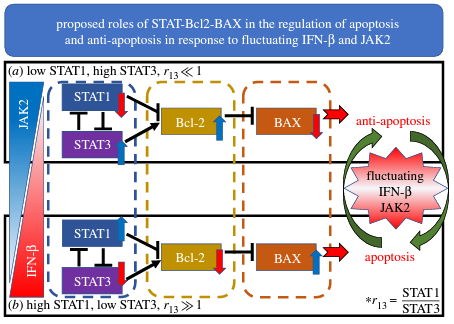
\includegraphics[width=0.75\textwidth]{Figures/stat.PNG}
		\end{framed}
	\caption{A schematic diagram for a proposed apoptosis signalling network in the presence of $IFN-\beta/JAK2$.\cite{lee2021mathematical}.}
	\label{fig:6}
\end{figure}

 
\subsection{Intracellular module of Signal Transducer and Activator of Transcription 1 (STAT1)}
\paragraph{}

The intracellular module of Signal Transducer and Activator of Transcription 1 (STAT1) is a protein that plays a key role in the body's immune response to viral infections. When activated, STAT1 binds to specific DNA sequences in the cell's genome, activating genes involved in the antiviral response. This includes the production of interferons and other cytokines, which help prevent the virus's spread throughout the body \cite{yang2021integrated}. Additionally, STAT1 can also inhibit the replication of certain viruses by blocking the activity of viral proteins. The intracellular module of STAT1 is activated by a variety of signalling pathways, including the Janus kinase (JAK) and phosphoinositide 3-kinase (PI3K) pathways. Dysregulation of STAT1 has been linked to a number of diseases, including cancer and autoimmune disorders. 

\subsection{Intracellular module of Signal Transducer and Activator of Transcription 3 (STAT3)}
\paragraph{}

The intracellular module of Signal Transducer and Activator of Transcription 3 (STAT3) is a protein that plays a key role in a variety of cellular processes, including cell growth, survival, and differentiation. According to the Human Protein Atlas project, the official gene symbol for STAT3 is "STAT3" \cite{stat3}, and the full gene name is "Signal transducer and activator of transcription 3". When activated, STAT3 binds to specific DNA sequences in the cell's genome, activating genes involved in cell growth, survival, and differentiation. It also plays a role in the inflammatory response, cell proliferation and differentiation. Also, when activated by certain cytokines, such as IL-11, IL-10, LIF, Oncostatin M and Leptin, STAT3 can enhance the Fas-mediated apoptosis of specific cells without any increase in cell surface Fas antigen expression \cite{tanaka2011stat3}. Furthermore, STAT3 siRNA transfection can suppress STAT3 expression and inhibit Fas-mediated cell death. [3] Dysregulation of STAT3 has been linked to a number of diseases, including cancer, autoimmune disorders, and others.

\subsection{Intracellular module of B-cell lymphoma 2 (Bcl-2)}
\paragraph{}

The intracellular module of B-cell lymphoma 2 (Bcl-2) is a family of proteins that play a key role in regulating the activation of the cell death program, also known as apoptosis. Some members of this family, like Bcl-2 itself or Bcl-XL, inhibit apoptosis by blocking the release of cytochrome c from mitochondria \cite{alberts2002programmed}. Bcl-2 proteins have been found in early metazoans including Porifera (sponges), Placozoans, and Cnidarians. Some viruses have gained Bcl-2 homologs and subvert innate immunity and cellular apoptosis for their replication, but they frequently have very different sequences to their host Bcl-2 analogues \cite{banjara2020bcl}. Intracellular flow cytometry can be used to measure the quantitative BCL-2 family protein abundance as a function of time and treatment to evaluate the mechanism(s) responsible for apoptotic triggering. Dysregulation of Bcl-2 family proteins has been linked to a number of diseases, including cancer, autoimmune disorders and others.

\subsection{Intracellular module of BCL-2-associated X protein (BAX)}
\paragraph{}

The intracellular module of BCL-2-associated X protein (BAX) is a protein that plays a key role in the regulation of the cell death program, also known as apoptosis. BAX is a member of the Bcl-2 family of proteins that promote apoptosis, in contrast to other members, such as Bcl-2 and Bcl-XL, which inhibit apoptosis. When BAX is activated, it oligomerizes and translocates to the mitochondria, where it can permeabilize the outer mitochondrial membrane and release pro-apoptotic factors such as cytochrome c \cite{andreu2017bax}. This leads to caspase activation, ultimately leading to cell degradation and death. BAX is activated by various signalling pathways, including the intrinsic and extrinsic pathways of apoptosis, and is regulated by other members of the Bcl-2 family, such as Bcl-2 and Bcl-XL. Dysregulation of BAX has been linked to a number of diseases, including cancer and neurodegenerative disorders \cite{czabotar2014control}. It's important to note that BAX is one of the vital proteins that initiate the cascade of events that leads to cell death via Apoptosis. It is a pro-apoptotic member of the Bcl-2 family of proteins, and its activation leads to the release of Cytochrome c from mitochondria, ultimately activating the cascade of caspases which leads to cell death.





\section{Mathematical model for intracellular module (STAT1, STAT3, Bcl-2 and BAX)}

\paragraph{}
The section should describe the mathematical models and techniques used to investigate the intracellular signalling network in more detail. First, a schematic diagram of the apoptosis signalling network will be described.   Key signalling network of apoptosis involving STAT1, STAT3, Bcl-2 and BAX in response to IFN-$\beta$ and JAK2 and the corresponding mathematical model: levels of STAT1 and STAT3 and activity of their target Bcl2 and BAX will be represented in more detail. 

\subsection{A schematic diagram of the apoptosis signalling network }
\paragraph{}

 \begin{figure}[hbt!]
	\centering
	\begin{framed}
	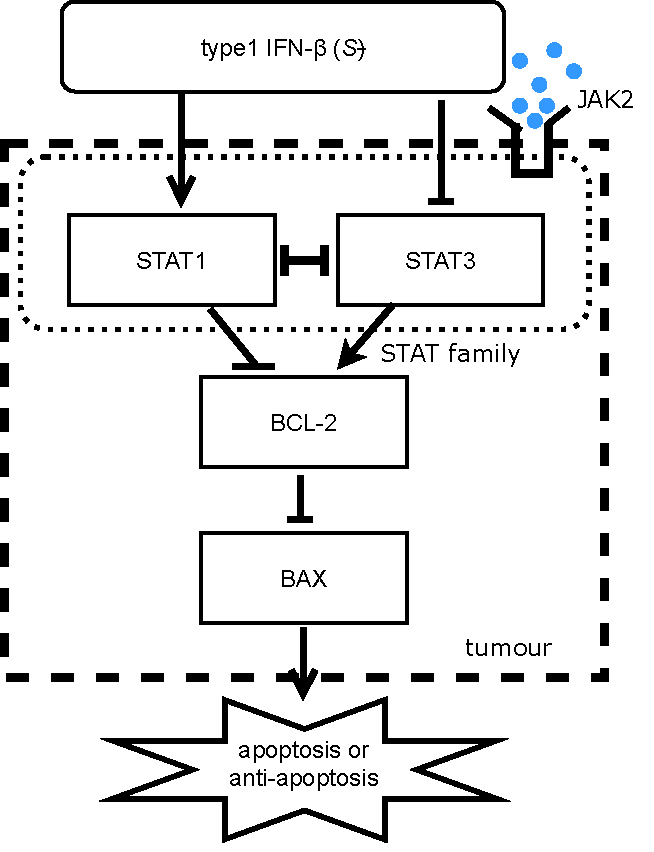
\includegraphics[width=0.7\textwidth]{Figures/D1.pdf}
		\end{framed}
	\caption{Key signalling network of apoptosis involving
STAT1, STAT3, Bcl-2 and BAX in response to IFN- $\beta$ and  JAK2  \cite{lee2021mathematical}.}
	\label{D1}
\end{figure}

 \begin{figure}[hbt!]
	\centering
	\begin{framed}
	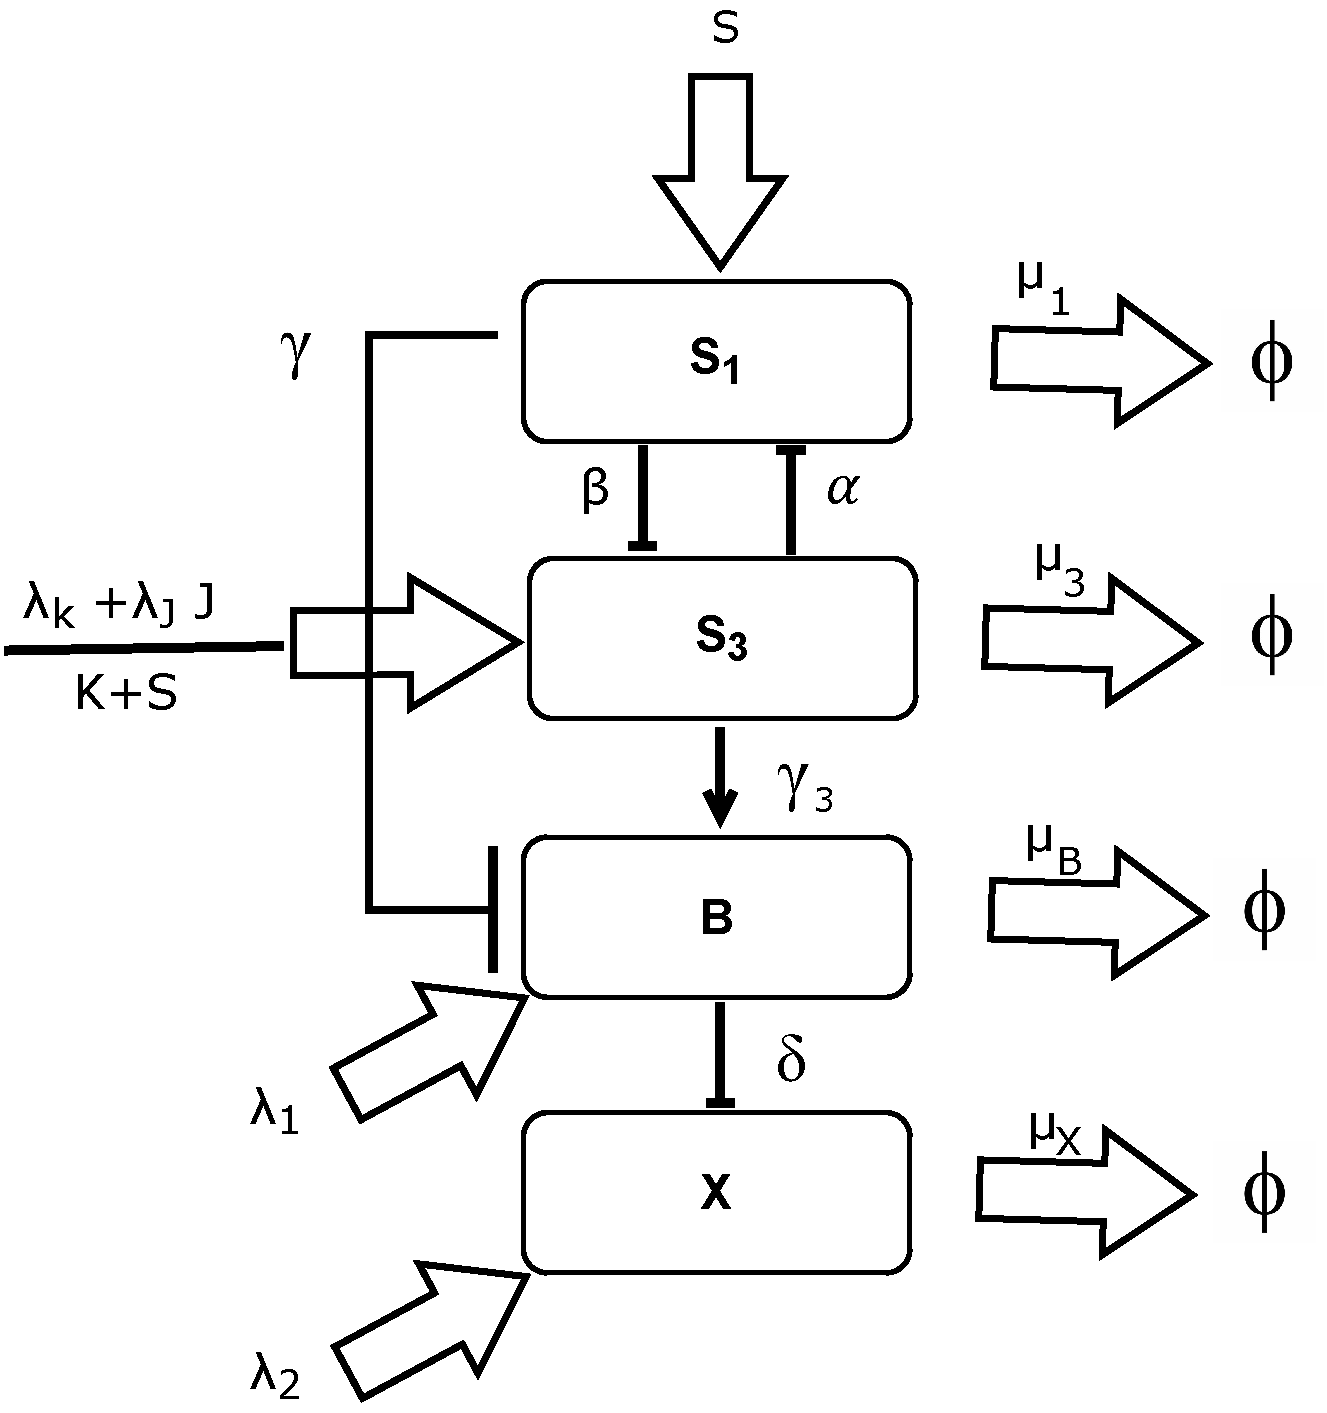
\includegraphics[width=0.7\textwidth]{Figures/D2.pdf}
		\end{framed}
	\caption{The corresponding mathematical model: levels of STAT1 and STAT3, and activity of their target Bcl2, and BAX were represented by ‘S1’, ‘S3’, ‘B’ and ‘X’, respectively \cite{lee2021mathematical}.}
	\label{D2}
\end{figure}

Figure \ref{D1} and Figure \ref{D2} is a schematic diagram that illustrates the apoptosis signalling network in response to IFN-$\beta$ and JAK2. Figure \ref{D1}, key signalling network of apoptosis: The figure illustrates the key signalling pathways involved in apoptosis, specifically the interactions between STAT1, STAT3, Bcl-2, and BAX in response to IFN-$\beta$ and JAK2. These proteins regulate the cell's response to stress, including the decision to undergo apoptosis. Figure \ref{D2},
the corresponding mathematical model: The figure also includes a mathematical representation of the signalling network. In this model, the levels of STAT1 and STAT3 are represented by 'S1' and 'S3' respectively, while the activity of their target proteins Bcl-2 and BAX are represented by 'B' and 'X' respectively. This mathematical representation mathematically models the interactions between these proteins and their responses to IFN-$\beta$ and JAK2 signalling. The model captures the dynamics of the interactions between the proteins, and allows for the prediction of the system's behavior.

Both Figure \ref{D1} and Figure \ref{D2} are representations of a mathematical model that captures the interactions of the key signalling pathways involved in apoptosis. It shows the critical signalling pathways, the proteins involved and their interactions, and the mathematical representation of the signalling network. This model allows the prediction of the system's behaviour.

\subsection{Governing ordinary differential equations (ODEs) for the intracellular signalling network}

\paragraph{}
The governing ordinary differential equations (ODEs) for the intracellular signalling network composed of STAT1, STAT3, Bcl-2, and BAX would likely be specific to the mathematical model used in a particular study. These ODEs would describe the dynamics of the concentrations of these proteins over time and would likely depend on various model parameters, such as rate constants for protein interactions and degradation.

 Let the variables $\Bar{S1}$, $\Bar{S3}$, $\Bar{B}$ and $\Bar{X}$ be concentrations of STAT1, STAT3, Bcl-2 and BAX at time $t$ respectively \cite{lee2021mathematical}. So then Then, the mass balance of the concentrations of STAT1 $\Bar{S1}$,  STAT3 $\Bar{S3}$, Bcl-2 $\Bar{B}$ and $\Bar{X}$ gives us. 

 
\begin{equation}
\label{a}
     \frac{d\Bar{S_1}}{dt} = f_{1} (s)+ \frac{ a_1a_2^2} {a_2^2+a_1F_1(\Bar{S_3})} - \mu_{s_{1}}\Bar{S_1 } 
\end{equation}

\begin{equation}
\label{b}
\frac{d\Bar{S_3}}{dt} = f_{2} (s.j)  +\frac{a_4a_5^2} {{a_5}^2+ a_6F_2({\Bar{S_3})}}-\mu_{s_{3}}\Bar{S_3} 
\end{equation}

\begin{equation}
\label{c}
\frac{d\Bar{B}}{dt} = f_3+ \frac{a_7a_8^2}{a_8^2+a_9F_3(\Bar{S_1})} -  \lambda_{STAT3} \Bar{S_3} - \mu_{Bcl2} \Bar{B} 
\end{equation}
 
\begin{equation}
\label{d}
    \frac{d \Bar{X}}{dt}= f_4 + \frac{a_10a_11^2}{a_11^2+a_12F_4(\Bar{X})} -\mu_X \Bar{X} 
\end{equation}

\newpage

The concentrations of $IFN$-$\beta$ and $JAK2$ are represented by $s$ and $j$, respectively. The rate of change in the concentration of STAT1 is determined by the input of $IFN-\beta$ through a function $f_1(s)$, the self-activating interaction with inhibition from STAT3 $(\Bar{S_3} \dashv \Bar{S_1})$ and the natural decrease in concentration at a rate $\mu_{S_1}$.  Each of ODEs equations explains the following details. 

\begin{itemize}
    \item In equation \eqref{a}, the high concentration of $IFN-\beta(s)$ upregulates the STAT1 level through the positive
function $f_1(s)$, while the high concentration of STAT3 inhibits the STAT1 level through the positive. 

\item The concentration of STAT3, represented in equation \eqref{b}, is influenced by signals from both $JAK$ and $IFN-\beta$ through a function $_2(s,j)$, self-activating interaction with inhibition from STAT1 $(\Bar{S_1} \dashv \Bar{S_3})$ and natural decrease in concentration at a rate $\mu_{S_3}$.

\item  Bcl-2 in equation \eqref{c} is regulated by the signal source at a fixed rate $f_3$, autocatalytic activity with inhibition from STAT1 $(\Bar{S_1} \dashv \Bar{B})$, upregulation from STAT3 $(\Bar{S_3} \dashv \Bar{B})$ at a rate $\lambda_{STAT3}$, and natural decay at a rate $\mu_{Bcl2}$.

\item In equation \eqref{d}, is regulated by the signal source at
a fixed rate $f_4$,  autocatalytic activity with inhibition from STAT1 $(\Bar{B} \dashv \Bar{X})$, and natural decrease in concentration at a rate $\mu_{BAX}$.
\end{itemize}

And also, we assume that, 

\begin{equation}
       f_1(s)=\lambda{IFN\beta s} , \quad    f_2(s,j)=\frac{K_2+\lambda{JAK}j}{K_1+\lambda{IFN\beta2s}}
\end{equation}

\begin{equation}
         F_1(\Bar{S_3})={\Bar{S_3}}^2 , \quad       F_2(\Bar{S_1})={\Bar{S_1}}^2, \quad  F_3(\Bar{S_1})={\Bar{S_1}}^2, \quad    F_4(\Bar{B})={\Bar{B}}^2
\end{equation}

where $\lambda_{IFN\beta}$ is the source of STAT1 from $IFN-\beta$, $\lambda_{IFN\beta2}$ is a source from $IFN-\beta$, and $\lambda_{JAK}$ is a source from JAK2. And also we use a non-dimensionalization formula as follows. 

\begin{equation}
\label{d1}
    t=\mu_{S_1}\Bar{t}, \quad     S_1=\frac{\Bar{S_1}}{{S_1}^*}, \quad S_3=\frac{\Bar{S_3}}{{S_3}^*}, \quad  B=\frac{\Bar{B}}{B^*}, \quad  X=\frac{\Bar{X}}{X^*}, \quad \mu_B=\frac{\mu_{Bcl2}}{\mu_{S_1}}, \quad \mu_X=\frac{\mu_{BAX}}{\mu_{S_1}}, \quad J=\frac{j}{J^*} \\

    k_1=\frac{a_1}{\mu_{s_1}{S_1}^*}, \quad  k_1=a_2, \quad \alpha=a_3({S_3}^*)^2, \quad  k_3=\frac{a_4}{\mu_{s_1}{S_3}^*}, \quad  k_4=a_5, \quad \beta=a_6({S_1}^*)^2, \quad \lambda_1=\frac{f_3}{\mu_{S_1}B^*} \\ 
    
    \lambda_2=\frac{f_4}{\mu_{S_1}X^*}, \quad  \lambda_k=\frac{K_2}{\mu_{S_1}{S_3}^*}, \quad \lambda_J=\frac{\lambda_{JAK}J^*}{\mu_{S_1}{S_3}*}, \quad \lambda_J=\frac{\lambda_{STAT3}{S_3}^*}{\mu_{S_1}B*}, \quad \lambda{S_1}=\frac{\lambda_{IFN\beta}S^*}{\mu_{S_1}{S_1}*}, \quad k_5=\frac{a_7}{\mu{S_1}B^*},\quad  k_2=a_2 \\
    
    k_7=\frac{a_10}{\mu{S_1}X^*}, \quad  k_6=a_8, \quad k_8=a_{11}, \quad k_4=a_5, \quad k_3=\frac{a_4}{\mu{S_1}{S_3}^*}, \quad \alpha=a_3({S_3}^*)^2, \gamma=a_9({S_1}^*)^2, \quad K=K_1\\
    
   \Lambda=a_12(X^*)^2 \quad S=\frac{s}{S^*}, \quad \beta=a_6({S_1}^*)^2, \quad \lambda_{S_2}=\lambda_{IFN\beta2}S^* \hspace{6cm}
\end{equation}


Then by using \eqref{d1} following governing equations were obtained. 

\begin{equation}
\label{e1}
     \frac{dS_1}{dt} = \lambda_{S_1} S + \frac{ k_1k_2^2} {k_2^2+\alpha S_3^2} - S_1  \\
\end{equation}

\begin{equation}
\label{e2}
\frac{dS_3}{dt} = \frac{\lambda_k+\lambda_JJ} {K+ \lambda_{S_2} S} +\frac{k_3{k_4}^2}{{k_4}^2+\beta{S_1}^2}-S_3 \\
\end{equation}

\begin{equation}
\label{e3}
\frac{dB}{dt} = \lambda_1+ \frac{k_5{k_6}^2}{{k_6}^2+\gamma{S_1}^2} -  \lambda_3 S_3 - \mu_BB \\
\end{equation}

\begin{equation}
\label{e4}
    \frac{dX}{dt}= \lambda_2+ \frac{k_7{k_8}^2}{{k_8}^2\Lambda B^2} -\mu_XX \\
\end{equation}

In the mathematical model of the kinetic network, as shown in figure 2b, the programmed cell death of cancer cells, also known as apoptosis, is triggered when the level of the anti-apoptotic protein Bcl-2 is lower than a certain threshold $(thB)$ and the level of the pro-apoptotic protein BAX is higher than another threshold $(thX)$. This is supported by experiments and previous modeling studies \cite{kim2019synergistic,bagci2006bistability,gaudette2016low}. The specific values of these thresholds were determined based on biological observations and the dynamic system of equations \eqref{e1},\eqref{e2},\eqref{e3} and \eqref{e4}.



\newpage

\section{Mathematical equilibrium and stability analysis}
\paragraph{}

The dynamics of the intracellular signalling system is governed by ordinary differential equations. 


\begin{equation}
\label{Q1}
     \frac{dS_1}{dt} = \lambda_{S_1} S + \frac{ k_1k_2^2} {k_2^2+\alpha S_3^2} - S_1  = H_1(S_1,S_3,B,X) \\
\end{equation}

\begin{equation}
\label{Q2}
\frac{dS_3}{dt} = \frac{\lambda_k+\lambda_JJ} {K+ \lambda_{S_2} S} +\frac{k_3{k_4}^2}{{k_4}^2+\beta{S_1}^2}-S_3  = H_2(S_1,S_3,B,X)\\
\end{equation}


\begin{equation}
\label{Q3}
\frac{dB}{dt} = \lambda_1+ \frac{k_5{k_6}^2}{{k_6}^2+\gamma{S_1}^2} -  \lambda_3 S_3 - \mu_BB = H_3(S_1,S_3,B,X)  \\
\end{equation}

\begin{equation}
\label{Q4}
    \frac{dX}{dt}= \lambda_2+ \frac{k_7{k_8}^2}{{k_8}^2\Lambda B^2} -\mu_XX = H_4(S_1,S_3,B,X) \\
\end{equation}

It is necessary to first identify the system's equilibrium state before exploring the equilibrium dynamics. This is accomplished by setting equations \eqref{Q1}, \eqref{Q2}, \eqref{Q3} and \eqref{Q4} to zero and performing the following calculations to find the answers $S_1^E, S_3^E, B^E$ and $X^E$:

\begin{equation}
\label{E1}
    S_1^E = \lambda_{S_1} S + \frac{ k_1k_2^2} {k_2^2+\alpha S_3^2} - S_1
\end{equation}

\begin{equation}
\label{E2}
S_3^E = \frac{\lambda_k+\lambda_JJ} {K+ \lambda_{S_2} S} +\frac{k_3{k_4}^2}{{k_4}^2+\beta{S_1}^2}-S_3  = H_2(S_1,S_3,B,X)\\
\end{equation}

\begin{equation}
\label{E3}
B^E = \lambda_1+ \frac{k_5{k_6}^2}{{k_6}^2+\gamma{S_1}^2} -  \lambda_3 S_3 - \mu_BB = H_3(S_1,S_3,B,X)  \\
\end{equation}

\begin{equation}
\label{E4}
    X^E= \lambda_2+ \frac{k_7{k_8}^2}{{k_8}^2\Lambda B^2} -\mu_XX = H_4(S_1,S_3,B,X) \\
\end{equation}
We can find the equilibrium point of the system \eqref{E1}-\eqref{E4} by nonlinear solver programming language as far as
all parameter values are fixed. 

The Jacobian matrix, J, is given by:
\begin{equation}
\label{s1}
    J = \begin{bmatrix}
\frac{\partial H1}{\partial S1} & \frac{\partial H1}{\partial S3} & \frac{\partial H1}{\partial B} & \frac{\partial H1}{\partial X} \\
\frac{\partial H2}{\partial S1} & \frac{\partial H2}{\partial S3} & \frac{\partial H2}{\partial B} & \frac{\partial H2}{\partial X} \\
\frac{\partial H3}{\partial S1} & \frac{\partial H3}{\partial S3} & \frac{\partial H3}{\partial B} & \frac{\partial H3}{\partial X} \\
\frac{\partial H4}{\partial S1} & \frac{\partial H4}{\partial S3} & \frac{\partial H4}{\partial B} & \frac{\partial H4}{\partial X}
\end{bmatrix}
\end{equation}

\begin{equation}
\label{s2}
    J = \begin{bmatrix}
-1 & -\frac{2k_1k_2^2\alpha SE_3^2}{(k_2^2 + \alpha(S_3^E)^2)^2} & 0 & 0 \\
-\frac{2k_3k_4^2\beta S_1^E}{(k_4^2+\beta(S_1^E)^2)^2} & -1 & 0 & 0 \\
-\frac{2k_5k_6^2\gamma(S_1^E)}{(k_6^2+\gamma (S_1^E)^2)} & -\lambda_3 & -\mu_B & 0 \\
0 & 0 & -\frac{2k_7k_8^2\Lambda B^E}{(k_8^2+\Lambda(B^E)^2)^2} & -\mu_X
\end{bmatrix}
\end{equation}

Then, the characteristic polynomial is given by 

\begin{equation}
\label{s3}
    (J - \Lambda I) = (\Lambda + \mu_B)(\Lambda + \mu_X) (\Lambda^2 + 2\Lambda +1 - \frac{2k_1k_2^2\alpha SE_3^2}{(k_2^2 + \alpha(S_3^E)^2)^2} \times \frac{2k_3k_4^2\beta S_1^E}{(k_4^2+\beta(S_1^E)^2)^2})
\end{equation}

Where I is the identity matrix. By using the above equations \eqref{s1}. \eqref{s2} and \eqref{s3} we can determine the stability of the system. 

 


\newpage




%\chapter{Methodology}
\label{chap:03}
\paragraph{}

The chapter provided a methodology  to discuss the involvement of the intracellular signalling network composed of STAT1, STAT3, Bcl-2, and BAX in regulating critical cellular states, including both anti-apoptosis and apoptosis of cancer cells, using Mathematical modeling. 
STAT1 plays a critical role in the control of T-cell homeostasis, and its suppressive/promoting role in tumorigenesis is influenced by environmental signals that might favour STAT1 activation in tumour cells or in host immune cells, respectively, with opposite consequences on tumour development. Interestingly, a mathematical framework will be adopted  to investigate how the STAT signalling pathways in cancer development and optimal control approaches can be modelled mathematically. And how intracellular module (STAT1, STAT3, Bcl-2 and BAX) dynamics play a key role in apoptotic cell death will be proved by using by illustrated results. This work will go over the intracellular module (STAT1, STAT3, Bcl-2 and BAX) ODEs system involving various situations and how they behave with different parameter values, as well as complex analysis using the Runge Kutta fourth order method and Euler's method and how to obtain the numerical analysis using software Java. Overall, these sources suggest that a mathematical approach is helpful in understanding the intracellular signalling network composed of STAT1, STAT3, Bcl-2, and BAX and its potential to be targeted for cancer therapy.


\newpage

\section{Biological approach of STAT1, STAT3, Bcl-2 and BAX}
\paragraph{}

The intracellular module (STAT1, STAT3, Bcl-2, and BAX) is a group of proteins that regulate various cellular processes, including cell growth, survival, and death. One approach to target these proteins is through the use of biologicals, such as drugs or other compounds that interact with these proteins to modulate their activity. One example of this is the use of niclosamide as a radiosensitizer in triple-negative breast cancer (TNBC) cells. Niclosamide was found to act by inhibiting STAT3 and Bcl-2 and increasing the generation of reactive oxygen species (ROS) in TNBC cells and xenograft tumours, leading to increased sensitivity to radiation therapy \cite{lu2018activation}. 

A mathematical model of STAT signalling pathways in cancer development and optimal control approaches was presented by Jonggul Lee, Donggu Lee 2 and Yangjin Kim in paper \cite{lee2021mathematical}. This model can be used to identify the potential targets for the biological approach in the treatment of cancer. It is worth mentioning that these proteins are complex and may have different effects in different contexts and cell types, so the biological approach should be tailored to the specific type of cancer and the stage of the disease. 

 \begin{figure}[hbt!]
	\centering
	\begin{framed}
	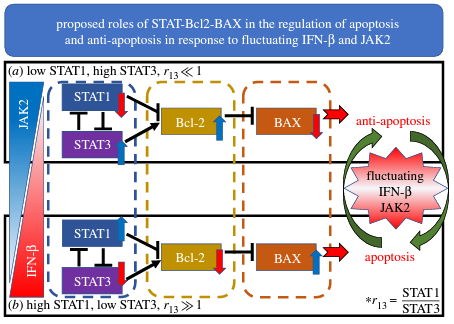
\includegraphics[width=0.75\textwidth]{Figures/stat.PNG}
		\end{framed}
	\caption{A schematic diagram for a proposed apoptosis signalling network in the presence of $IFN-\beta/JAK2$.\cite{lee2021mathematical}.}
	\label{fig:6}
\end{figure}

 
\subsection{Intracellular module of Signal Transducer and Activator of Transcription 1 (STAT1)}
\paragraph{}

The intracellular module of Signal Transducer and Activator of Transcription 1 (STAT1) is a protein that plays a key role in the body's immune response to viral infections. When activated, STAT1 binds to specific DNA sequences in the cell's genome, activating genes involved in the antiviral response. This includes the production of interferons and other cytokines, which help prevent the virus's spread throughout the body \cite{yang2021integrated}. Additionally, STAT1 can also inhibit the replication of certain viruses by blocking the activity of viral proteins. The intracellular module of STAT1 is activated by a variety of signalling pathways, including the Janus kinase (JAK) and phosphoinositide 3-kinase (PI3K) pathways. Dysregulation of STAT1 has been linked to a number of diseases, including cancer and autoimmune disorders. 

\subsection{Intracellular module of Signal Transducer and Activator of Transcription 3 (STAT3)}
\paragraph{}

The intracellular module of Signal Transducer and Activator of Transcription 3 (STAT3) is a protein that plays a key role in a variety of cellular processes, including cell growth, survival, and differentiation. According to the Human Protein Atlas project, the official gene symbol for STAT3 is "STAT3" \cite{stat3}, and the full gene name is "Signal transducer and activator of transcription 3". When activated, STAT3 binds to specific DNA sequences in the cell's genome, activating genes involved in cell growth, survival, and differentiation. It also plays a role in the inflammatory response, cell proliferation and differentiation. Also, when activated by certain cytokines, such as IL-11, IL-10, LIF, Oncostatin M and Leptin, STAT3 can enhance the Fas-mediated apoptosis of specific cells without any increase in cell surface Fas antigen expression \cite{tanaka2011stat3}. Furthermore, STAT3 siRNA transfection can suppress STAT3 expression and inhibit Fas-mediated cell death. [3] Dysregulation of STAT3 has been linked to a number of diseases, including cancer, autoimmune disorders, and others.

\subsection{Intracellular module of B-cell lymphoma 2 (Bcl-2)}
\paragraph{}

The intracellular module of B-cell lymphoma 2 (Bcl-2) is a family of proteins that play a key role in regulating the activation of the cell death program, also known as apoptosis. Some members of this family, like Bcl-2 itself or Bcl-XL, inhibit apoptosis by blocking the release of cytochrome c from mitochondria \cite{alberts2002programmed}. Bcl-2 proteins have been found in early metazoans including Porifera (sponges), Placozoans, and Cnidarians. Some viruses have gained Bcl-2 homologs and subvert innate immunity and cellular apoptosis for their replication, but they frequently have very different sequences to their host Bcl-2 analogues \cite{banjara2020bcl}. Intracellular flow cytometry can be used to measure the quantitative BCL-2 family protein abundance as a function of time and treatment to evaluate the mechanism(s) responsible for apoptotic triggering. Dysregulation of Bcl-2 family proteins has been linked to a number of diseases, including cancer, autoimmune disorders and others.

\subsection{Intracellular module of BCL-2-associated X protein (BAX)}
\paragraph{}

The intracellular module of BCL-2-associated X protein (BAX) is a protein that plays a key role in the regulation of the cell death program, also known as apoptosis. BAX is a member of the Bcl-2 family of proteins that promote apoptosis, in contrast to other members, such as Bcl-2 and Bcl-XL, which inhibit apoptosis. When BAX is activated, it oligomerizes and translocates to the mitochondria, where it can permeabilize the outer mitochondrial membrane and release pro-apoptotic factors such as cytochrome c \cite{andreu2017bax}. This leads to caspase activation, ultimately leading to cell degradation and death. BAX is activated by various signalling pathways, including the intrinsic and extrinsic pathways of apoptosis, and is regulated by other members of the Bcl-2 family, such as Bcl-2 and Bcl-XL. Dysregulation of BAX has been linked to a number of diseases, including cancer and neurodegenerative disorders \cite{czabotar2014control}. It's important to note that BAX is one of the vital proteins that initiate the cascade of events that leads to cell death via Apoptosis. It is a pro-apoptotic member of the Bcl-2 family of proteins, and its activation leads to the release of Cytochrome c from mitochondria, ultimately activating the cascade of caspases which leads to cell death.





\section{Mathematical model for intracellular module (STAT1, STAT3, Bcl-2 and BAX)}

\paragraph{}
The section should describe the mathematical models and techniques used to investigate the intracellular signalling network in more detail. First, a schematic diagram of the apoptosis signalling network will be described.   Key signalling network of apoptosis involving STAT1, STAT3, Bcl-2 and BAX in response to IFN-$\beta$ and JAK2 and the corresponding mathematical model: levels of STAT1 and STAT3 and activity of their target Bcl2 and BAX will be represented in more detail. 

\subsection{A schematic diagram of the apoptosis signalling network }
\paragraph{}

 \begin{figure}[hbt!]
	\centering
	\begin{framed}
	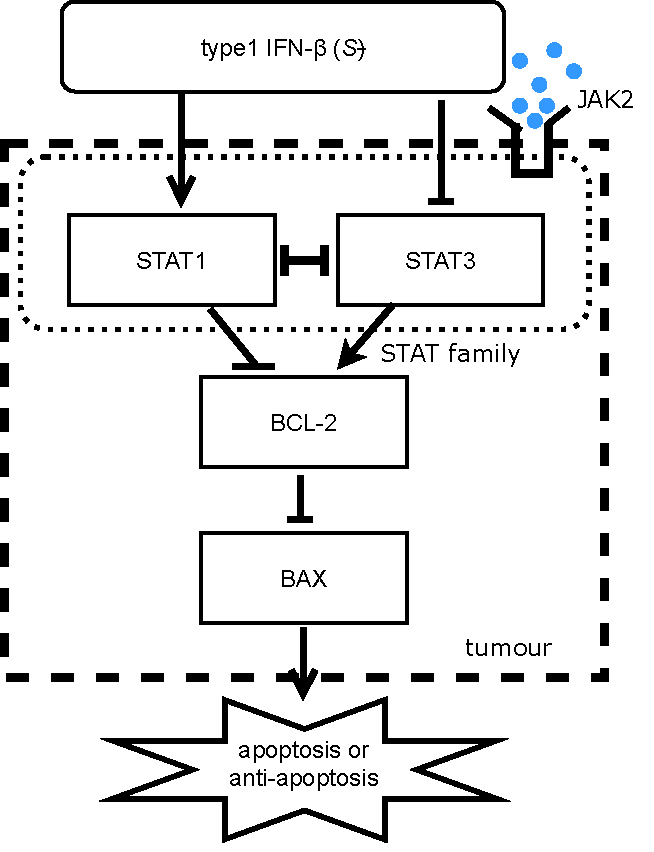
\includegraphics[width=0.7\textwidth]{Figures/D1.pdf}
		\end{framed}
	\caption{Key signalling network of apoptosis involving
STAT1, STAT3, Bcl-2 and BAX in response to IFN- $\beta$ and  JAK2  \cite{lee2021mathematical}.}
	\label{D1}
\end{figure}

 \begin{figure}[hbt!]
	\centering
	\begin{framed}
	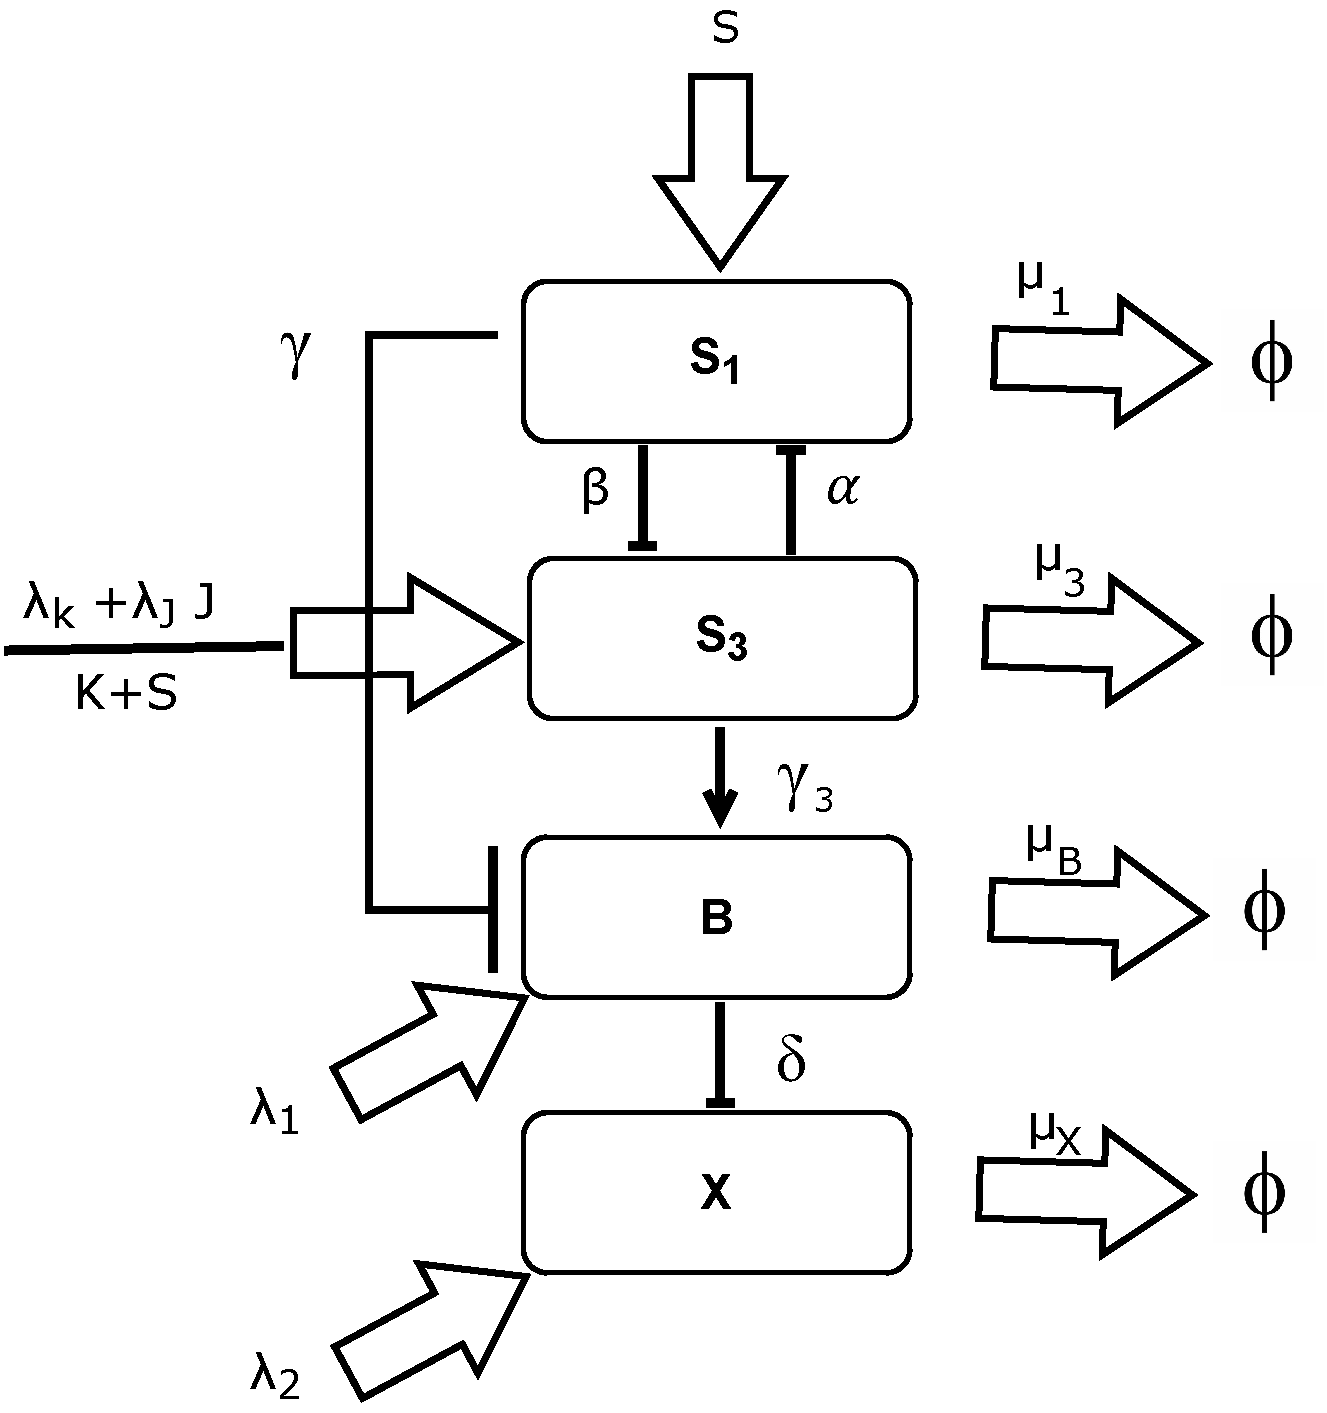
\includegraphics[width=0.7\textwidth]{Figures/D2.pdf}
		\end{framed}
	\caption{The corresponding mathematical model: levels of STAT1 and STAT3, and activity of their target Bcl2, and BAX were represented by ‘S1’, ‘S3’, ‘B’ and ‘X’, respectively \cite{lee2021mathematical}.}
	\label{D2}
\end{figure}

Figure \ref{D1} and Figure \ref{D2} is a schematic diagram that illustrates the apoptosis signalling network in response to IFN-$\beta$ and JAK2. Figure \ref{D1}, key signalling network of apoptosis: The figure illustrates the key signalling pathways involved in apoptosis, specifically the interactions between STAT1, STAT3, Bcl-2, and BAX in response to IFN-$\beta$ and JAK2. These proteins regulate the cell's response to stress, including the decision to undergo apoptosis. Figure \ref{D2},
the corresponding mathematical model: The figure also includes a mathematical representation of the signalling network. In this model, the levels of STAT1 and STAT3 are represented by 'S1' and 'S3' respectively, while the activity of their target proteins Bcl-2 and BAX are represented by 'B' and 'X' respectively. This mathematical representation mathematically models the interactions between these proteins and their responses to IFN-$\beta$ and JAK2 signalling. The model captures the dynamics of the interactions between the proteins, and allows for the prediction of the system's behavior.

Both Figure \ref{D1} and Figure \ref{D2} are representations of a mathematical model that captures the interactions of the key signalling pathways involved in apoptosis. It shows the critical signalling pathways, the proteins involved and their interactions, and the mathematical representation of the signalling network. This model allows the prediction of the system's behaviour.

\subsection{Governing ordinary differential equations (ODEs) for the intracellular signalling network}

\paragraph{}
The governing ordinary differential equations (ODEs) for the intracellular signalling network composed of STAT1, STAT3, Bcl-2, and BAX would likely be specific to the mathematical model used in a particular study. These ODEs would describe the dynamics of the concentrations of these proteins over time and would likely depend on various model parameters, such as rate constants for protein interactions and degradation.

 Let the variables $\Bar{S1}$, $\Bar{S3}$, $\Bar{B}$ and $\Bar{X}$ be concentrations of STAT1, STAT3, Bcl-2 and BAX at time $t$ respectively \cite{lee2021mathematical}. So then Then, the mass balance of the concentrations of STAT1 $\Bar{S1}$,  STAT3 $\Bar{S3}$, Bcl-2 $\Bar{B}$ and $\Bar{X}$ gives us. 

 
\begin{equation}
\label{a}
     \frac{d\Bar{S_1}}{dt} = f_{1} (s)+ \frac{ a_1a_2^2} {a_2^2+a_1F_1(\Bar{S_3})} - \mu_{s_{1}}\Bar{S_1 } 
\end{equation}

\begin{equation}
\label{b}
\frac{d\Bar{S_3}}{dt} = f_{2} (s.j)  +\frac{a_4a_5^2} {{a_5}^2+ a_6F_2({\Bar{S_3})}}-\mu_{s_{3}}\Bar{S_3} 
\end{equation}

\begin{equation}
\label{c}
\frac{d\Bar{B}}{dt} = f_3+ \frac{a_7a_8^2}{a_8^2+a_9F_3(\Bar{S_1})} -  \lambda_{STAT3} \Bar{S_3} - \mu_{Bcl2} \Bar{B} 
\end{equation}
 
\begin{equation}
\label{d}
    \frac{d \Bar{X}}{dt}= f_4 + \frac{a_10a_11^2}{a_11^2+a_12F_4(\Bar{X})} -\mu_X \Bar{X} 
\end{equation}

\newpage

The concentrations of $IFN$-$\beta$ and $JAK2$ are represented by $s$ and $j$, respectively. The rate of change in the concentration of STAT1 is determined by the input of $IFN-\beta$ through a function $f_1(s)$, the self-activating interaction with inhibition from STAT3 $(\Bar{S_3} \dashv \Bar{S_1})$ and the natural decrease in concentration at a rate $\mu_{S_1}$.  Each of ODEs equations explains the following details. 

\begin{itemize}
    \item In equation \eqref{a}, the high concentration of $IFN-\beta(s)$ upregulates the STAT1 level through the positive
function $f_1(s)$, while the high concentration of STAT3 inhibits the STAT1 level through the positive. 

\item The concentration of STAT3, represented in equation \eqref{b}, is influenced by signals from both $JAK$ and $IFN-\beta$ through a function $_2(s,j)$, self-activating interaction with inhibition from STAT1 $(\Bar{S_1} \dashv \Bar{S_3})$ and natural decrease in concentration at a rate $\mu_{S_3}$.

\item  Bcl-2 in equation \eqref{c} is regulated by the signal source at a fixed rate $f_3$, autocatalytic activity with inhibition from STAT1 $(\Bar{S_1} \dashv \Bar{B})$, upregulation from STAT3 $(\Bar{S_3} \dashv \Bar{B})$ at a rate $\lambda_{STAT3}$, and natural decay at a rate $\mu_{Bcl2}$.

\item In equation \eqref{d}, is regulated by the signal source at
a fixed rate $f_4$,  autocatalytic activity with inhibition from STAT1 $(\Bar{B} \dashv \Bar{X})$, and natural decrease in concentration at a rate $\mu_{BAX}$.
\end{itemize}

And also, we assume that, 

\begin{equation}
       f_1(s)=\lambda{IFN\beta s} , \quad    f_2(s,j)=\frac{K_2+\lambda{JAK}j}{K_1+\lambda{IFN\beta2s}}
\end{equation}

\begin{equation}
         F_1(\Bar{S_3})={\Bar{S_3}}^2 , \quad       F_2(\Bar{S_1})={\Bar{S_1}}^2, \quad  F_3(\Bar{S_1})={\Bar{S_1}}^2, \quad    F_4(\Bar{B})={\Bar{B}}^2
\end{equation}

where $\lambda_{IFN\beta}$ is the source of STAT1 from $IFN-\beta$, $\lambda_{IFN\beta2}$ is a source from $IFN-\beta$, and $\lambda_{JAK}$ is a source from JAK2. And also we use a non-dimensionalization formula as follows. 

\begin{equation}
\label{d1}
    t=\mu_{S_1}\Bar{t}, \quad     S_1=\frac{\Bar{S_1}}{{S_1}^*}, \quad S_3=\frac{\Bar{S_3}}{{S_3}^*}, \quad  B=\frac{\Bar{B}}{B^*}, \quad  X=\frac{\Bar{X}}{X^*}, \quad \mu_B=\frac{\mu_{Bcl2}}{\mu_{S_1}}, \quad \mu_X=\frac{\mu_{BAX}}{\mu_{S_1}}, \quad J=\frac{j}{J^*} \\

    k_1=\frac{a_1}{\mu_{s_1}{S_1}^*}, \quad  k_1=a_2, \quad \alpha=a_3({S_3}^*)^2, \quad  k_3=\frac{a_4}{\mu_{s_1}{S_3}^*}, \quad  k_4=a_5, \quad \beta=a_6({S_1}^*)^2, \quad \lambda_1=\frac{f_3}{\mu_{S_1}B^*} \\ 
    
    \lambda_2=\frac{f_4}{\mu_{S_1}X^*}, \quad  \lambda_k=\frac{K_2}{\mu_{S_1}{S_3}^*}, \quad \lambda_J=\frac{\lambda_{JAK}J^*}{\mu_{S_1}{S_3}*}, \quad \lambda_J=\frac{\lambda_{STAT3}{S_3}^*}{\mu_{S_1}B*}, \quad \lambda{S_1}=\frac{\lambda_{IFN\beta}S^*}{\mu_{S_1}{S_1}*}, \quad k_5=\frac{a_7}{\mu{S_1}B^*},\quad  k_2=a_2 \\
    
    k_7=\frac{a_10}{\mu{S_1}X^*}, \quad  k_6=a_8, \quad k_8=a_{11}, \quad k_4=a_5, \quad k_3=\frac{a_4}{\mu{S_1}{S_3}^*}, \quad \alpha=a_3({S_3}^*)^2, \gamma=a_9({S_1}^*)^2, \quad K=K_1\\
    
   \Lambda=a_12(X^*)^2 \quad S=\frac{s}{S^*}, \quad \beta=a_6({S_1}^*)^2, \quad \lambda_{S_2}=\lambda_{IFN\beta2}S^* \hspace{6cm}
\end{equation}


Then by using \eqref{d1} following governing equations were obtained. 

\begin{equation}
\label{e1}
     \frac{dS_1}{dt} = \lambda_{S_1} S + \frac{ k_1k_2^2} {k_2^2+\alpha S_3^2} - S_1  \\
\end{equation}

\begin{equation}
\label{e2}
\frac{dS_3}{dt} = \frac{\lambda_k+\lambda_JJ} {K+ \lambda_{S_2} S} +\frac{k_3{k_4}^2}{{k_4}^2+\beta{S_1}^2}-S_3 \\
\end{equation}

\begin{equation}
\label{e3}
\frac{dB}{dt} = \lambda_1+ \frac{k_5{k_6}^2}{{k_6}^2+\gamma{S_1}^2} -  \lambda_3 S_3 - \mu_BB \\
\end{equation}

\begin{equation}
\label{e4}
    \frac{dX}{dt}= \lambda_2+ \frac{k_7{k_8}^2}{{k_8}^2\Lambda B^2} -\mu_XX \\
\end{equation}

In the mathematical model of the kinetic network, as shown in figure 2b, the programmed cell death of cancer cells, also known as apoptosis, is triggered when the level of the anti-apoptotic protein Bcl-2 is lower than a certain threshold $(thB)$ and the level of the pro-apoptotic protein BAX is higher than another threshold $(thX)$. This is supported by experiments and previous modeling studies \cite{kim2019synergistic,bagci2006bistability,gaudette2016low}. The specific values of these thresholds were determined based on biological observations and the dynamic system of equations \eqref{e1},\eqref{e2},\eqref{e3} and \eqref{e4}.



\newpage

\section{Mathematical equilibrium and stability analysis}
\paragraph{}

The dynamics of the intracellular signalling system is governed by ordinary differential equations. 


\begin{equation}
\label{Q1}
     \frac{dS_1}{dt} = \lambda_{S_1} S + \frac{ k_1k_2^2} {k_2^2+\alpha S_3^2} - S_1  = H_1(S_1,S_3,B,X) \\
\end{equation}

\begin{equation}
\label{Q2}
\frac{dS_3}{dt} = \frac{\lambda_k+\lambda_JJ} {K+ \lambda_{S_2} S} +\frac{k_3{k_4}^2}{{k_4}^2+\beta{S_1}^2}-S_3  = H_2(S_1,S_3,B,X)\\
\end{equation}


\begin{equation}
\label{Q3}
\frac{dB}{dt} = \lambda_1+ \frac{k_5{k_6}^2}{{k_6}^2+\gamma{S_1}^2} -  \lambda_3 S_3 - \mu_BB = H_3(S_1,S_3,B,X)  \\
\end{equation}

\begin{equation}
\label{Q4}
    \frac{dX}{dt}= \lambda_2+ \frac{k_7{k_8}^2}{{k_8}^2\Lambda B^2} -\mu_XX = H_4(S_1,S_3,B,X) \\
\end{equation}

It is necessary to first identify the system's equilibrium state before exploring the equilibrium dynamics. This is accomplished by setting equations \eqref{Q1}, \eqref{Q2}, \eqref{Q3} and \eqref{Q4} to zero and performing the following calculations to find the answers $S_1^E, S_3^E, B^E$ and $X^E$:

\begin{equation}
\label{E1}
    S_1^E = \lambda_{S_1} S + \frac{ k_1k_2^2} {k_2^2+\alpha S_3^2} - S_1
\end{equation}

\begin{equation}
\label{E2}
S_3^E = \frac{\lambda_k+\lambda_JJ} {K+ \lambda_{S_2} S} +\frac{k_3{k_4}^2}{{k_4}^2+\beta{S_1}^2}-S_3  = H_2(S_1,S_3,B,X)\\
\end{equation}

\begin{equation}
\label{E3}
B^E = \lambda_1+ \frac{k_5{k_6}^2}{{k_6}^2+\gamma{S_1}^2} -  \lambda_3 S_3 - \mu_BB = H_3(S_1,S_3,B,X)  \\
\end{equation}

\begin{equation}
\label{E4}
    X^E= \lambda_2+ \frac{k_7{k_8}^2}{{k_8}^2\Lambda B^2} -\mu_XX = H_4(S_1,S_3,B,X) \\
\end{equation}
We can find the equilibrium point of the system \eqref{E1}-\eqref{E4} by nonlinear solver programming language as far as
all parameter values are fixed. 

The Jacobian matrix, J, is given by:
\begin{equation}
\label{s1}
    J = \begin{bmatrix}
\frac{\partial H1}{\partial S1} & \frac{\partial H1}{\partial S3} & \frac{\partial H1}{\partial B} & \frac{\partial H1}{\partial X} \\
\frac{\partial H2}{\partial S1} & \frac{\partial H2}{\partial S3} & \frac{\partial H2}{\partial B} & \frac{\partial H2}{\partial X} \\
\frac{\partial H3}{\partial S1} & \frac{\partial H3}{\partial S3} & \frac{\partial H3}{\partial B} & \frac{\partial H3}{\partial X} \\
\frac{\partial H4}{\partial S1} & \frac{\partial H4}{\partial S3} & \frac{\partial H4}{\partial B} & \frac{\partial H4}{\partial X}
\end{bmatrix}
\end{equation}

\begin{equation}
\label{s2}
    J = \begin{bmatrix}
-1 & -\frac{2k_1k_2^2\alpha SE_3^2}{(k_2^2 + \alpha(S_3^E)^2)^2} & 0 & 0 \\
-\frac{2k_3k_4^2\beta S_1^E}{(k_4^2+\beta(S_1^E)^2)^2} & -1 & 0 & 0 \\
-\frac{2k_5k_6^2\gamma(S_1^E)}{(k_6^2+\gamma (S_1^E)^2)} & -\lambda_3 & -\mu_B & 0 \\
0 & 0 & -\frac{2k_7k_8^2\Lambda B^E}{(k_8^2+\Lambda(B^E)^2)^2} & -\mu_X
\end{bmatrix}
\end{equation}

Then, the characteristic polynomial is given by 

\begin{equation}
\label{s3}
    (J - \Lambda I) = (\Lambda + \mu_B)(\Lambda + \mu_X) (\Lambda^2 + 2\Lambda +1 - \frac{2k_1k_2^2\alpha SE_3^2}{(k_2^2 + \alpha(S_3^E)^2)^2} \times \frac{2k_3k_4^2\beta S_1^E}{(k_4^2+\beta(S_1^E)^2)^2})
\end{equation}

Where I is the identity matrix. By using the above equations \eqref{s1}. \eqref{s2} and \eqref{s3} we can determine the stability of the system. 

 


\newpage




\chapter{Numerical Method for Ordinary Differential Equations}
\label{chap:04}

\paragraph{}


Differential equations are a powerful tool for describing systems that are changing over time. They are used in a wide range of fields, including science and engineering, economics, social science, biology, business, and health care. Mathematicians have developed many techniques for understanding and solving these equations, and many complex systems can be precisely described using these mathematical tools.

However, many systems are so complex or so large that a purely mathematical description is not possible. In these cases, computer simulations and numerical approximations can be used to better understand the system. Before the advent of programmable computers, solving differential equations required large teams of people working with mechanical calculators. Today, however, the increased speed and power of computers has made it possible to solve even the most complex systems of differential equations on a single machine. 

In this section, we will discuss some of the fundamental strategies and techniques for solving differential equations using Java. We will start by looking at the basics of differential equations for intracellular signalling networks (STAT1, STAT3, Bcl-2 and
BAX). Then, we will introduce two popular numerical methods for solving these equations: the Runge-Kutta fourth-order method and Euler's method. These methods allow us to obtain numerical results for the systems we are studying, even if a purely mathematical solution is not possible. Overall, this section provides an overview of how to use differential equations and numerical methods to understand complex systems. 



\section{Numerical investigation using Euler's method}
\label{sec:4.1}
\paragraph{}

In this section, all the details about numerical analysis using Euler's method for the as earlier stated, four differential equations ( equation \eqref{e1}, \eqref{e2}, \eqref{e3} and  \eqref{aac}) will be discussed. Euler's method is a simple and popular technique for numerically solving ordinary differential equations (ODEs). To use Euler's method to solve the equations above, you would follow these steps:

\begin{enumerate}
    \item Set the initial conditions for each variable in the equations, such as $S_1(0)$, $S_3(0)$, $B(0)$, and $X(0)$.
    \item Choose a step size (often denoted as $h$) and a time interval over which you want to solve the equations, such as $0$ to $10$ seconds with a step size of $0.1$ seconds.
    \item Iterate over the time interval, updating the value of each variable at each step using the following formula:

    \begin{equation}
        S_1(t + h) = S_1(t) + h * \frac{dS_1}{dt}
    \end{equation}

    \begin{equation}
        S_3(t + h) = S_3(t) + h * \frac{dS_3}{dt}
    \end{equation}

      \begin{equation}
        B(t + h) = B(t) + h * \frac{dB}{dt}
    \end{equation}

      \begin{equation}
        X(t + h) = X(t) + h * \frac{dX}{dt}
    \end{equation}

    Where the right-hand side of each of these equations is evaluated using the current values of the variables and the parameters in the equations.

\item Repeat step 3 until you have reached the end of the time interval. The resulting values of each variable at each time step will be an approximation of the proper solution to the equations.
 
\end{enumerate}


 Note that Euler's method is first-order, meaning that the approximation error increases as the step size decreases. Therefore, the solution may not be accurate for small step sizes. You can use higher-order methods such as the Runge-Kutta method to improve the accuracy.

\section{ Numerical integration technique for Runge-Kutta fourth order method}
\paragraph{}

The Runge-Kutta fourth-order method (also known as the RK4 method) is a numerical method for solving ordinary differential equations (ODEs). The basic idea behind the method is to approximate the solution of the ODE at a given time step by using a weighted average of four estimates of the solution at that time step, each estimate being based on a different approximation of the derivative of the solution at that time step.

The Runge-Kutta fourth-order method (also known as the RK4 method) is a numerical method for solving ordinary differential equations (ODEs). The basic idea behind the method is to approximate the solution of the ODE at a given time step by using a weighted average of four estimates of the solution at that time step, each estimate being based on a different approximation of the derivative of the solution at that time step.

Once you have the initial conditions and time step specified, you would then use the following procedure to solve the ODEs:

\begin{enumerate}
    \item Set the initial values of $S_1$, $S_3$, $B$, and $X$ to their initial conditions.
    \item For each time step, starting from the initial time, repeat the following steps:

    \begin{itemize}
        \item Compute the derivatives of $S_1$, $S_3$, $B$, and $X$ at the current time step using equations (\eqref{e1})-(\eqref{e4}).

        \item Use the derivatives to compute the following estimates of the solution at the next time step:

\begin{equation}
     - S_1^1 = \Delta t \left(\lambda_{S_1} S + \frac{ k_1k_2^2} {k_2^2+\alpha S_3^2} - S_1\right)
\end{equation}

\begin{equation}
      - S_3^1 = \Delta t \left( \frac{\lambda_k+\lambda_JJ} {K+ \lambda_{S_2} S} +\frac{k_3{k_4}^2}{{k_4}^2+\beta{S_1}^2}-S_3\right)
\end{equation}

\begin{equation}
    - B^1 = \Delta t\left( \lambda_1+ \frac{k_5{k_6}^2}{{k_6}^2+\gamma{S_1}^2} -  \lambda_3 S_3 - \mu_BB\right)
\end{equation}
    
\begin{equation}
     - X^1 = \Delta t\left(\lambda_2+ \frac{k_7{k_8}^2}{{k_8}^2\delta B^2} -\mu_XX\right)
\end{equation}

\item Compute the derivatives of $S_1$, $S_3$, $B$, and $X$ at the next time step using equations (\eqref{e1})-(\eqref{e4}) and the estimates obtained in step 2b. 

\begin{equation}
     - S_1^2 = \Delta t \left(\lambda_{S_1} (S+S_1^1/2) + \frac{ k_1k_2^2} {k_2^2+\alpha (S_3+S_3^1/2)^2} - (S_1+S_1^1/2)\right)
\end{equation}

\begin{equation}
 -S_3^2 = \Delta t \left( \frac{\lambda_k+\lambda_JJ} {K+ \lambda_{S_2} (S+S_1^1/2)} +\frac{k_3{k_4}^2}{{k_4}^2+\beta(S_1+S_1^1/2)^2}-(S_3+S_3^1/2) \right
\end{equation}

\begin{equation}
    -B^2 = \Delta t \left( \lambda_1+ \frac{k_5{k_6}^2}{{k_6}^2+\gamma(S_1+S_1^1/2)^2} - \lambda_3 (S_3+S_3^1/2) - \mu_B (B+B^1/2)\right)
\end{equation}

\begin{equation}
    -X^2 = \Delta t \left( \lambda_2+ \frac{k_7{k_8}^2}{{k_8}^2\delta (B+B^1/2)^2} -\mu_X (X+X^1/2)\right)
\end{equation}

    \end{itemize}

\item Using the initial conditions and the ODEs (equations \eqref{e1}, \eqref{e2}, \eqref{e3}, and \eqref{e4}), compute the values of k1, k2, k3, and k4 for each variable at the current time step.

\begin{equation}
    k1 = h * (\lambda_{S_1} S + \frac{ k_1k_2^2} {k_2^2+\alpha S_3^2} - S_1)
\end{equation}

\begin{equation}
    k2 = h * (\frac{\lambda_k+\lambda_JJ} {K+ \lambda_{S_2} S} +\frac{k_3{k_4}^2}{{k_4}^2+\beta{S_1}^2}-S_3)
\end{equation}

\begin{equation}
    k3 = h * (\lambda_1+ \frac{k_5{k_6}^2}{{k_6}^2+\gamma{S_1}^2} - \lambda_3 S_3 - \mu_BB)
\end{equation}

\begin{equation}
    k4 = h * (\lambda_2+ \frac{k_7{k_8}^2}{{k_8}^2\delta B^2} -\mu_XX)
\end{equation}

\item Compute the new values of S1, S3, B, and X at the next time step using the following formulas:

\begin{equation}
    S_1(t+h) = S_1(t) + \frac{1}{6}(k1 + 2k2 + 2k3 + k4)
\end{equation}

\begin{equation}
    S_3(t+h) = S_3(t) + \frac{1}{6}(k1 + 2k2 + 2k3 + k4)
\end{equation}

\begin{equation}
    B(t+h) = B(t) + \frac{1}{6}(k1 + 2k2 + 2k3 + k4)
\end{equation}

\begin{equation}
    B(t+h) = B(t) + \frac{1}{6}(k1 + 2k2 + 2k3 + k4)
\end{equation}

\item Repeat steps 3 and 4 for each time step until the end of the simulation. 
\end{enumerate}

It's important to note that the specific values of k1, k2, k3, and k4 will depend on the values of the variables at the current time step and on the specific ODEs being solved.


%\chapter{Numerical Method for Ordinary Differential Equations}
\label{chap:04}

\paragraph{}


Differential equations are a powerful tool for describing systems that are changing over time. They are used in a wide range of fields, including science and engineering, economics, social science, biology, business, and health care. Mathematicians have developed many techniques for understanding and solving these equations, and many complex systems can be precisely described using these mathematical tools.

However, many systems are so complex or so large that a purely mathematical description is not possible. In these cases, computer simulations and numerical approximations can be used to better understand the system. Before the advent of programmable computers, solving differential equations required large teams of people working with mechanical calculators. Today, however, the increased speed and power of computers has made it possible to solve even the most complex systems of differential equations on a single machine. 

In this section, we will discuss some of the fundamental strategies and techniques for solving differential equations using Java. We will start by looking at the basics of differential equations for intracellular signalling networks (STAT1, STAT3, Bcl-2 and
BAX). Then, we will introduce two popular numerical methods for solving these equations: the Runge-Kutta fourth-order method and Euler's method. These methods allow us to obtain numerical results for the systems we are studying, even if a purely mathematical solution is not possible. Overall, this section provides an overview of how to use differential equations and numerical methods to understand complex systems. 



\section{Numerical investigation using Euler's method}
\label{sec:4.1}
\paragraph{}

In this section, all the details about numerical analysis using Euler's method for the as earlier stated, four differential equations ( equation \eqref{e1}, \eqref{e2}, \eqref{e3} and  \eqref{aac}) will be discussed. Euler's method is a simple and popular technique for numerically solving ordinary differential equations (ODEs). To use Euler's method to solve the equations above, you would follow these steps:

\begin{enumerate}
    \item Set the initial conditions for each variable in the equations, such as $S_1(0)$, $S_3(0)$, $B(0)$, and $X(0)$.
    \item Choose a step size (often denoted as $h$) and a time interval over which you want to solve the equations, such as $0$ to $10$ seconds with a step size of $0.1$ seconds.
    \item Iterate over the time interval, updating the value of each variable at each step using the following formula:

    \begin{equation}
        S_1(t + h) = S_1(t) + h * \frac{dS_1}{dt}
    \end{equation}

    \begin{equation}
        S_3(t + h) = S_3(t) + h * \frac{dS_3}{dt}
    \end{equation}

      \begin{equation}
        B(t + h) = B(t) + h * \frac{dB}{dt}
    \end{equation}

      \begin{equation}
        X(t + h) = X(t) + h * \frac{dX}{dt}
    \end{equation}

    Where the right-hand side of each of these equations is evaluated using the current values of the variables and the parameters in the equations.

\item Repeat step 3 until you have reached the end of the time interval. The resulting values of each variable at each time step will be an approximation of the proper solution to the equations.
 
\end{enumerate}


 Note that Euler's method is first-order, meaning that the approximation error increases as the step size decreases. Therefore, the solution may not be accurate for small step sizes. You can use higher-order methods such as the Runge-Kutta method to improve the accuracy.

\section{ Numerical integration technique for Runge-Kutta fourth order method}
\paragraph{}

The Runge-Kutta fourth-order method (also known as the RK4 method) is a numerical method for solving ordinary differential equations (ODEs). The basic idea behind the method is to approximate the solution of the ODE at a given time step by using a weighted average of four estimates of the solution at that time step, each estimate being based on a different approximation of the derivative of the solution at that time step.

The Runge-Kutta fourth-order method (also known as the RK4 method) is a numerical method for solving ordinary differential equations (ODEs). The basic idea behind the method is to approximate the solution of the ODE at a given time step by using a weighted average of four estimates of the solution at that time step, each estimate being based on a different approximation of the derivative of the solution at that time step.

Once you have the initial conditions and time step specified, you would then use the following procedure to solve the ODEs:

\begin{enumerate}
    \item Set the initial values of $S_1$, $S_3$, $B$, and $X$ to their initial conditions.
    \item For each time step, starting from the initial time, repeat the following steps:

    \begin{itemize}
        \item Compute the derivatives of $S_1$, $S_3$, $B$, and $X$ at the current time step using equations (\eqref{e1})-(\eqref{e4}).

        \item Use the derivatives to compute the following estimates of the solution at the next time step:

\begin{equation}
     - S_1^1 = \Delta t \left(\lambda_{S_1} S + \frac{ k_1k_2^2} {k_2^2+\alpha S_3^2} - S_1\right)
\end{equation}

\begin{equation}
      - S_3^1 = \Delta t \left( \frac{\lambda_k+\lambda_JJ} {K+ \lambda_{S_2} S} +\frac{k_3{k_4}^2}{{k_4}^2+\beta{S_1}^2}-S_3\right)
\end{equation}

\begin{equation}
    - B^1 = \Delta t\left( \lambda_1+ \frac{k_5{k_6}^2}{{k_6}^2+\gamma{S_1}^2} -  \lambda_3 S_3 - \mu_BB\right)
\end{equation}
    
\begin{equation}
     - X^1 = \Delta t\left(\lambda_2+ \frac{k_7{k_8}^2}{{k_8}^2\delta B^2} -\mu_XX\right)
\end{equation}

\item Compute the derivatives of $S_1$, $S_3$, $B$, and $X$ at the next time step using equations (\eqref{e1})-(\eqref{e4}) and the estimates obtained in step 2b. 

\begin{equation}
     - S_1^2 = \Delta t \left(\lambda_{S_1} (S+S_1^1/2) + \frac{ k_1k_2^2} {k_2^2+\alpha (S_3+S_3^1/2)^2} - (S_1+S_1^1/2)\right)
\end{equation}

\begin{equation}
 -S_3^2 = \Delta t \left( \frac{\lambda_k+\lambda_JJ} {K+ \lambda_{S_2} (S+S_1^1/2)} +\frac{k_3{k_4}^2}{{k_4}^2+\beta(S_1+S_1^1/2)^2}-(S_3+S_3^1/2) \right
\end{equation}

\begin{equation}
    -B^2 = \Delta t \left( \lambda_1+ \frac{k_5{k_6}^2}{{k_6}^2+\gamma(S_1+S_1^1/2)^2} - \lambda_3 (S_3+S_3^1/2) - \mu_B (B+B^1/2)\right)
\end{equation}

\begin{equation}
    -X^2 = \Delta t \left( \lambda_2+ \frac{k_7{k_8}^2}{{k_8}^2\delta (B+B^1/2)^2} -\mu_X (X+X^1/2)\right)
\end{equation}

    \end{itemize}

\item Using the initial conditions and the ODEs (equations \eqref{e1}, \eqref{e2}, \eqref{e3}, and \eqref{e4}), compute the values of k1, k2, k3, and k4 for each variable at the current time step.

\begin{equation}
    k1 = h * (\lambda_{S_1} S + \frac{ k_1k_2^2} {k_2^2+\alpha S_3^2} - S_1)
\end{equation}

\begin{equation}
    k2 = h * (\frac{\lambda_k+\lambda_JJ} {K+ \lambda_{S_2} S} +\frac{k_3{k_4}^2}{{k_4}^2+\beta{S_1}^2}-S_3)
\end{equation}

\begin{equation}
    k3 = h * (\lambda_1+ \frac{k_5{k_6}^2}{{k_6}^2+\gamma{S_1}^2} - \lambda_3 S_3 - \mu_BB)
\end{equation}

\begin{equation}
    k4 = h * (\lambda_2+ \frac{k_7{k_8}^2}{{k_8}^2\delta B^2} -\mu_XX)
\end{equation}

\item Compute the new values of S1, S3, B, and X at the next time step using the following formulas:

\begin{equation}
    S_1(t+h) = S_1(t) + \frac{1}{6}(k1 + 2k2 + 2k3 + k4)
\end{equation}

\begin{equation}
    S_3(t+h) = S_3(t) + \frac{1}{6}(k1 + 2k2 + 2k3 + k4)
\end{equation}

\begin{equation}
    B(t+h) = B(t) + \frac{1}{6}(k1 + 2k2 + 2k3 + k4)
\end{equation}

\begin{equation}
    B(t+h) = B(t) + \frac{1}{6}(k1 + 2k2 + 2k3 + k4)
\end{equation}

\item Repeat steps 3 and 4 for each time step until the end of the simulation. 
\end{enumerate}

It's important to note that the specific values of k1, k2, k3, and k4 will depend on the values of the variables at the current time step and on the specific ODEs being solved.


\chapter{Results and Discussion}
\label{chap:05}
\paragraph{}

The Runge-Kutta fourth-order method  and Euler's method can be used to optimize and improve the performance of the intracellular signalling network for the STAT1, STAT3, BCL-2 and BAX proteins. This method can be used to determine the relationship between the initial conditions and other parameters of the proteins, such as anti-tumour drugs in the presence of IFN-$\beta$ and JAK stimuli. By doing so, the dynamic characteristics of the proteins can be predicted under different conditions and calculated using the numerical method of Runge-Kutta fourth order and Euler's method. This allows for precise \cite{lee2021mathematical}imation of the proteins' dynamic characteristics during their movement processes and adequate description of the different processes under various given conditions. The results obtained using this method, such as  the presence of IFN-$\beta$ and JAK and other effective parameters, provide valuable insights into the behaviour of the STAT1, STAT3, BCL-2 and BAX proteins.


\begin{table}[hbt!]
\begin{center}
    \begin{tabular}{p{2cm}|p{6cm}|p{3cm}}
    \hline
    \textbf{Constant} & \textbf{Description of constant} & \textbf{Values}
    \\
    \hline \hline
 ${S_1}^*$&STAT1 concentration&2.42 $\mu g ml^{-1}$\\
${S_3}^*$&STAT3 concentration&1.38 $\mu g ml^{-1}$\\
$B^*$&Bcl-2 concentration&10 nM \\
$X^*$&BAX concentration&351  $\mu$M\\
$S^*$&IFN-$\beta$ concentration&10 $ng ml^{-1}$\\
$J^*$&JAK2 concentration&10 nM\\
$D^*$&DDP concentration&10 $\mu g ml^{-1}$\\
$T^*$&tumour volume&$100mm^3$\\
     \hline
    \end{tabular}
    \caption{Initial values corresponding to the STAT1, STAT3, Bcl-2, BAX and other parameters.  }
    \label{tab1}
    \end{center}
\end{table}

% For future illustration, above Table\ref{tab1} values will be used. Each iteration calculated will be calculated using step size and time. 

 \begin{table}[hbt!]
\begin{center}
    \begin{tabular}{p{2.5cm}|p{9cm}|p{1.2cm}|p{2cm}}
    \hline
  \textbf{Constant} &  \textbf{Description of constant} &\textbf{Values} &\textbf{Reference}
    \\
    \hline \hline
    S & IFN-$\beta$ signalling  & 0-1.0& \cite{lee2021mathematical,deng2014sting}\\
$k_1$ & autocatalytic production rate(STAT1 module) & 4.0 & \cite{lee2021mathematical}\\
$ k_2$ & Hill-type coefficient (STAT1 module) & 1.0  & \cite{lee2021mathematical}\\
   $\alpha$ & inhibition strength of STAT1 by STAT3 & 1.5 & \cite{lee2021mathematical}\\
   $\lambda_k $& signalling source of STAT3 & 1.0 & \cite{lee2021mathematical}\\
   $ \lambda_J$ & induction rate of STAT3 by JAK2 & 4.0 & \cite{lee2021mathematical}\\
      J & JAK2 signalling level & 0-1.0 & \cite{lee2021mathematical}\\
K & inhibition parameter & 5.0 & \cite{lee2021mathematical}\\
$k_3$ & autocatalytic production rate (STAT3 module) & 4.0 & \cite{lee2021mathematical}\\
$k_4$ & Hill-type coefficient (STAT3 module) & 1.0 & \cite{lee2021mathematical}\\
$\beta$ & inhibition strength of STAT3 by STAT1& 1.0 & \cite{lee2021mathematical}\\
$\mu_3$ & relative decay rate of STAT3 & 1.0 & \cite{andrejeva2002degradation, yang2017porcine}\\
$\lambda_1$ & signalling source of Bcl-2 & 0.2 & \cite{lee2021mathematical}\\
$k_5$ & autocatalytic production rate (Bcl-2 module) & 1.0 & \cite{lee2021mathematical}\\
$k_6$ & Hill-type coefficient (Bcl-2 module) & 1.0 & \cite{lee2021mathematical}\\
$\gamma $ & inhibition strength of Bcl-2 by STAT$1_1$ & 1.0 & \cite{lee2021mathematical}\\
$\lambda_3$ & signalling from STAT3 & 1.2 & \cite{lee2021mathematical}\\
$\mu_B$ & relative decay rate of Bcl-2 & 1.2 &  \cite{andrejeva2002degradation, yang2017porcine}\\
$\lambda_2$ & signalling source of BAX& 0.2 & \cite{lee2021mathematical}\\
$k_7$ & autocatalytic production rate (BAX module) & 4.0 & \cite{lee2021mathematical}\\
$k_8$ & Hill-type coefficient (BAX module) & 1.0 & \cite{lee2021mathematical}\\
$\Lambda$ & inhibition strength of BAX by Bcl-2& 1.0 & \cite{lee2021mathematical}\\
$\mu_X$ & relative decay rate of BAX & 5.0& \cite{magal2005downregulation, xin2005nicotine}\\
\textbf{Threshold} & & & \\ 
\hline
 ${S_1}^{th}$ & threshold of STAT1  & 1.8& \cite{lee2021mathematical}\\
 ${S_3}^{th}$ & threshold of STAT3  & 1.3& \cite{lee2021mathematical}\\
 $B^{th}$ & threshold of Bcl-2  & 1.44& \cite{lee2021mathematical}\\
 $X^{th}$ & threshold of BAX  & 0.3& \cite{lee2021mathematical}\\
\textbf{Tumour module} & & &\\
     \hline
 r& growth rate of tumour cells& 0.12&\cite{catani2016intratumoral}\\
 ${k_9}$& inhibition parameter of STAT1 growth& 1.0&\cite{catani2016intratumoral}\\
 ${k_{10}}$& inhibition parameter of STAT1 growth& 10&\cite{catani2016intratumoral}\\
 ${T_0}$& carrying capacity of a tumour&100&\cite{catani2016intratumoral}\\
${\mu_T}$& killing rate of tumour cells by apoptosis&0.1&\cite{catani2016intratumoral}\\
 \hline
    \end{tabular}
    \caption{Values of the constant corresponding to the mathematical model. }
    \label{tabR1}
    \end{center}
\end{table}

Dynamic behaviour of STAT1, STAT3, BCL-2, and BAX systems optimized and analyzed using Runge-Kutta and Euler's method using Table \ref{tabR1} and Table \ref{tabR2}.

\newpage


 \begin{table}[hbt!]
\begin{center}
    \begin{tabular}{p{2.5cm}|p{6cm}|p{2cm}|p{2cm}}
    \hline
  \textbf{Constant} &  \textbf{Description of constant} &\textbf{Values} &\textbf{Reference}
    \\
    \hline \hline
\textbf{Therapeutics}& & &\\
 ${\mu_S}$& decay rate of IFN-$\beta$ &4.8& \cite{salmon1996pharmacokinetics}\\
 ${J_s}$& source of JAK2&1.3& \cite{lin2008fc}\\
 ${\mu_J}$& decay rate of JAK2 &1.3& \cite{lin2008fc}\\
 ${\gamma_D}$& degradation rate of JAK2 by DDP &1.0& \cite{lee2021mathematical}\\
     ${\mu_D}$&decay rate of DDP &10& \cite{crom1981cisplatin}\\
\textbf{Reference value}& & &\\
${S_1}^*$&STAT1 concentration&2.42 $\mu g ml^{-1}$& \cite{liu2014active}\\
${S_3}^*$&STAT3 concentration&1.38 $\mu g ml^{-1}$&\cite{liu2014active}\\
$B^*$&Bcl-2 concentration&10 nM & \cite{vickers2017animal}\\
$X^*$&BAX concentration&351  $\mu$M &\cite{vickers2017animal}\\
$S^*$&IFN-$\beta$ concentration&10 $ng ml^{-1}$& \cite{yu2009transcriptional}\\
$J^*$&JAK2 concentration&10 nM& \cite{lee2021mathematical,yu2009transcriptional}\\
$D^*$&DDP concentration&10 $\mu g ml^{-1}$&\cite{lee2021mathematical}\\
$T^*$&tumour volume&$100mm^3$&\cite{lee2021mathematical}\\
 \hline
    \end{tabular}
    \caption{Values of the constant corresponding to the mathematical model.}
    \label{tabR2}
    \end{center}
\end{table}


\section{Numerical results for $S =0$ and $J=0$}
\paragraph{}

This section discusses the behaviour of intracellular modules (STAT1, STAT3, Bcl-2, and BAX) using Euler's method and Runge Kutta fourth-order method. The behaviour of each module is depicted in figures, with solid, dashed, dotted, and dot-dashed lines representing STAT1, STAT3, Bcl-2, and BAX, respectively. Comparison results for each module are also shown in separate figures for clarity. The dynamics of STAT1, STAT3, and Bcl-2 are consistent with the numerical results of both Euler's and the Runge Kutta methods.

In Figure \ref{r2} the behaviour of intracellular module (STAT1, STAT3, Bcl-2, and BAX) using Runge kutta fourth order method. Using Figues \ref{r1} and Figure \ref{r2} it is challenging to refer to changes in their behaviours. Therefore, comparison result of each module (STAT1, STAT3, Bcl-2, and BAX) can be shown in Figures \ref{r3}, \ref{r4}, \ref{r5} and \ref{r6}. The dynamics of STAT1  (Figure \ref{r3}) STAT3  (Figure \ref{r4}) and Bcl-2 (Figure \ref{r5}) have coincided of their results corresponding to the numerical result of Runge Kutta method and Euler's method.  

\begin{figure}[hbt!]
	\centering
	\begin{framed}
	\includegraphics[width=0.68\textwidth]{Figures/A/N1.png}
		\end{framed}
	\caption{Numerical results by Euler's method when $S =0$ and $J=0$.}
	\label{r1}
\end{figure}


\begin{figure}[hbt!]
	\centering
	\begin{framed}
	\includegraphics[width=0.68\textwidth]{Figures/A/N2.png}
		\end{framed}
	\caption{Numerical results by Runge kutta fourth order method  when $S =0$ and $J=0$. }
	\label{r2}
\end{figure}

\begin{figure}[hbt!]
	\centering
	\begin{framed}
	\includegraphics[width=0.68\textwidth]{Figures/A/N3.png}
		\end{framed}
	\caption{STAT1 behavior corresponding to the RK4 method and Euler's method  when $S =0$ and $J=0$.}
	\label{r3}
\end{figure}
 
\begin{figure}[hbt!]
	\centering
	\begin{framed}
	\includegraphics[width=0.67\textwidth]{Figures/A/N4.png}
		\end{framed}
	\caption{STAT3 behavior corresponding to the RK4 method and Euler's method  when $S =0$ and $J=0$.}
	\label{r4}
\end{figure}

\begin{figure}[hbt!]
	\centering
	\begin{framed}
	\includegraphics[width=0.67\textwidth]{Figures/A/N5.png}
		\end{framed}
	\caption{Bcl-2 behavior corresponding to the RK4 method and Euler's method  when $S =0$ and $J=0$.}
	\label{r5}
\end{figure}

\begin{figure}[hbt!]
	\centering
	\begin{framed}
	\includegraphics[width=0.67\textwidth]{Figures/A/N6.png}
		\end{framed}
	\caption{BAX behavior corresponding to the RK4 method and Euler's method  when $S =0$ and $J=0$.}
	\label{r6}
\end{figure}





\section{Numerical results for $S =0.4$ and $J=0$}
\paragraph{}
 
In this section, there are several scenarios will be discussed with analysis results. Results will be interpreted corresponding to the $S =0.4$ and $J=0$  values and initial values as given in Table \ref{tab1}. Figure \ref{r13} depicts the behaviour of the intracellular module (STAT1, STAT3, Bcl-2, and BAX) using Euler's method and Runge kutta fourth order method. Each and every intracellular module (STAT1, STAT3, Bcl-2, and BAX) starts in different initial conditions and then they are decremented into several values. The solid, dashed, dotted, and dot-dashed lines represent the STAT1, STAT3, Bcl-2, and BAX, respectively. 

In Figure \ref{r14} the behaviour of intracellular module (STAT1, STAT3, Bcl-2, and BAX) using Runge kutta fourth order method. Using Figues \ref{r13} and Figure \ref{r14}, it is challenging to refer to changes in their behaviours. Therefore, comparison result of each module (STAT1, STAT3, Bcl-2, and BAX) can be shown in Figures \ref{r15}, \ref{r16}, \ref{r17} and \ref{r18}. The dynamics of STAT1  (Figure \ref{r15}) STAT3  (Figure \ref{r16}) and Bcl-2 (Figure \ref{r17}) have coincided with their results corresponding to the numerical result of Runge Kutta method and Euler's method.

 \begin{figure}[hbt!]
	\centering
	\begin{framed}
	\includegraphics[width=0.68\textwidth]{Figures/C/N1.png}
		\end{framed}
	\caption{Numerical results  by Euler's method when $S =0.4$ and $J=0$.}
	\label{r13}
\end{figure}

\begin{figure}[hbt!]
	\centering
	\begin{framed}
	\includegraphics[width=0.68\textwidth]{Figures/C/N2.png}
		\end{framed}
	\caption{Numerical results  by Runge kutta fouth order method when $S =0.4$ and $J=0$. }
	\label{r14}
\end{figure}

\begin{figure}[hbt!]
	\centering
	\begin{framed}
	\includegraphics[width=0.68\textwidth]{Figures/C/N3.png}
		\end{framed}
	\caption{STAT1 behavior corresponding to the RK4 method and Euler's method when $S =0.4$ and $J=0$.}
	\label{r15}
\end{figure}

\begin{figure}[hbt!]
	\centering
	\begin{framed}
	\includegraphics[width=0.68\textwidth]{Figures/C/N4.png}
		\end{framed}
	\caption{STAT3 behavior corresponding to the RK4 method and Euler's method when $S =0.4$ and $J=0$.}
	\label{r16}
\end{figure}

\begin{figure}[hbt!]
	\centering
	\begin{framed}
	\includegraphics[width=0.68\textwidth]{Figures/C/N5.png}
		\end{framed}
	\caption{Bcl-2 behavior corresponding to the RK4 method and Euler's method when $S =0.4$ and $J=0$.}
	\label{r17}
\end{figure}

\begin{figure}[hbt!]
	\centering
	\begin{framed}
	\includegraphics[width=0.68\textwidth]{Figures/C/N6.png}
		\end{framed}
	\caption{BAX behavior corresponding to the RK4 method and Euler's method when $S =0.4$ and $J=0$.}
	\label{r18}
\end{figure}

\section{Numerical results for $S =1$ and $J=1$}
\paragraph{}


In this section, the presence of both IFN-$\beta$ signalling and JAK2 signalling levels will be examined through analysis of results. The interpretation of the results will be based on the values of $S=1$ and $J=1$ as listed in Table 1. Figures \ref{r19}  and \ref{r20}  show the behaviour of the intracellular modules (STAT1, STAT3, Bcl-2, and BAX) using both Euler's method and the Runge-Kutta fourth-order method, respectively. The initial conditions for each of the modules were set as given in Table \ref{tab1}. The figures' solid line, dashed line, dotted line, and dot-dashed line represent the behaviour of STAT1, STAT3, Bcl-2, and BAX, respectively. To better understand the changes in their behaviour, comparison results for each module can be found in Figures \ref{r21}, \ref{r22}, \ref{r23} and \ref{r24}. The dynamics of STAT1  (Figure \ref{r21}) STAT3  (Figure \ref{r22}) and Bcl-2 (Figure \ref{r23}) have coincided of their results corresponding to the numerical result of Runge-Kutta method and Euler's method. The dynamics of STAT1, STAT3, and Bcl-2 are consistent with the numerical results obtained from both Runge-Kutta and Euler's method.  

\newpage

 \begin{figure}[hbt!]
	\centering
	\begin{framed}
	\includegraphics[width=0.68\textwidth]{Figures/D/N1.png}
		\end{framed}
	\caption{Numerical results  by Euler's method when $S =1$ and $J=1$.}
	\label{r19}
\end{figure}

\begin{figure}[hbt!]
	\centering
	\begin{framed}
	\includegraphics[width=0.68\textwidth]{Figures/D/N2.png}
		\end{framed}
	\caption{Numerical results  by Runge kutta fouth order method when $S =1$ and $J=1$. }
	\label{r20}
\end{figure}

\begin{figure}[hbt!]
	\centering
	\begin{framed}
	\includegraphics[width=0.68\textwidth]{Figures/D/N3.png}
		\end{framed}
	\caption{STAT1 behavior corresponding to the RK4 method and Euler's method when $S =1$ and $J=1$.}
	\label{r21}
\end{figure}

\begin{figure}[hbt!]
	\centering
	\begin{framed}
	\includegraphics[width=0.68\textwidth]{Figures/D/N4.png}
		\end{framed}
	\caption{STAT3 behavior corresponding to the RK4 method and Euler's method when $S =1$ and $J=1$.}
	\label{r22}
\end{figure}

\begin{figure}[hbt!]
	\centering
	\begin{framed}
	\includegraphics[width=0.68\textwidth]{Figures/D/N5.png}
		\end{framed}
	\caption{Bcl-2 behavior corresponding to the RK4 method and Euler's method when $S =1$ and $J=1$.}
	\label{r23}
\end{figure}

\begin{figure}[hbt!]
	\centering
	\begin{framed}
	\includegraphics[width=0.68\textwidth]{Figures/D/N6.png}
		\end{framed}
	\caption{BAX behavior corresponding to the RK4 method and Euler's method when $S =1$ and $J=1$.}
	\label{r24}
\end{figure}

\section{Equilibrium and stability analysis}
\paragraph{}

This section will be described the equilibrium and stability analysis
corresponding to the mathematical model. 

considering the Jacobean matrix for the equations, 

\begin{equation}
\label{s1}
    J = \begin{bmatrix}
\frac{\partial H1}{\partial S1} & \frac{\partial H1}{\partial S3} & \frac{\partial H1}{\partial B} & \frac{\partial H1}{\partial X} \\
\frac{\partial H2}{\partial S1} & \frac{\partial H2}{\partial S3} & \frac{\partial H2}{\partial B} & \frac{\partial H2}{\partial X} \\
\frac{\partial H3}{\partial S1} & \frac{\partial H3}{\partial S3} & \frac{\partial H3}{\partial B} & \frac{\partial H3}{\partial X} \\
\frac{\partial H4}{\partial S1} & \frac{\partial H4}{\partial S3} & \frac{\partial H4}{\partial B} & \frac{\partial H4}{\partial X}
\end{bmatrix}
\end{equation}

\begin{equation}
\label{se2}
    J = \begin{bmatrix}
-1 & -\frac{2k_1k_2^2\alpha SE_3^2}{(k_2^2 + \alpha(S_3^E)^2)^2} & 0 & 0 \\
-\frac{2k_3k_4^2\beta S_1^E}{(k_4^2+\beta(S_1^E)^2)^2} & -1 & 0 & 0 \\
-\frac{2k_5k_6^2\gamma(S_1^E)}{(k_6^2+\gamma (S_1^E)^2)} & -\lambda_3 & -\mu_B & 0 \\
0 & 0 & -\frac{2k_7k_8^2\Lambda B^E}{(k_8^2+\Lambda(B^E)^2)^2} & -\mu_X
\end{bmatrix}
\end{equation}

Then, the characteristic polynomial is given by

\begin{equation}
\label{s3}
    (J - \Lambda I) = (\Lambda + \mu_B)(\Lambda + \mu_X) (\Lambda^2 + 2\Lambda +1 - \frac{2k_1k_2^2\alpha SE_3^2}{(k_2^2 + \alpha(S_3^E)^2)^2} \times \frac{2k_3k_4^2\beta S_1^E}{(k_4^2+\beta(S_1^E)^2)^2})
\end{equation}

Where I is the identity matrix. By suing above equations \eqref{s1}. \eqref{s2} and \eqref{s3} we can determine the stability of the system. We get two real eigenvalues $(\Lambda_1 = -\mu_B < 0$ and $\Lambda_2 = - \mu_X < 0)$. And remaining two real eigenvalues are,

\begin{equation}
    \Lambda_{3,4} = -1 \pm \sqrt{\frac{2k_1k_2^2\alpha SE_3^2}{(k_2^2 + \alpha(S_3^E)^2)^2} \times \frac{2k_3k_4^2\beta S_1^E}{(k_4^2+\beta(S_1^E)^2)^2}}
\end{equation}

If $\frac{2k_1k_2^2\alpha SE_3^2}{(k_2^2 + \alpha(S_3^E)^2)^2} \times \frac{2k_3k_4^2\beta S_1^E}{(k_4^2+\beta(S_1^E)^2)^2} < 1$ the eigenvalues $\Lambda_{3,4}$ are negative and the equilibrium is stable. And also, if if $\frac{2k_1k_2^2\alpha SE_3^2}{(k_2^2 + \alpha(S_3^E)^2)^2} \times \frac{2k_3k_4^2\beta S_1^E}{(k_4^2+\beta(S_1^E)^2)^2} > 1$  then $\Lambda_{3,4} > 0$ and the equilibrium is unstable. 

By substituting parameter values in the model to \eqref{se2} , we get,

\begin{equation}
    \label{re1}
     J = \begin{bmatrix}
-1 & -\frac{12 SE_3^2}{(1 + 1.5(S_3^E)^2)^2} & 0 & 0 \\
-\frac{8 S_1^E}{(1+(S_1^E)^2)^2} & -1 & 0 & 0 \\
-\frac{2(S_1^E)}{(1+\gamma (S_1^E)^2)} & 1.2 & -1.2 & 0 \\
0 & 0 & -\frac{8 B^E}{(1+\Lambda(B^E)^2)^2} & -5
\end{bmatrix}
\end{equation}

By setting $A =  -\frac{12 SE_3^2}{(1 + 1.5(S_3^E)^2)^2}$, $B = -\frac{8 S_1^E}{(1+(S_1^E)^2)^2} $, $C = -\frac{2(S_1^E)}{(1+\gamma (S_1^E)^2)} $ and $D =  -\frac{8 B^E}{(1+\Lambda(B^E)^2)^2}$

\begin{equation}
    \label{re1}
     J = \begin{bmatrix}
-1 & A& 0 & 0 \\
B & -1 & 0 & 0 \\
C & 1.2 & -1.2 & 0 \\
0 & 0 &D & -5
\end{bmatrix}
\end{equation}

Then, the characteristic equation is

\begin{equation}
    (J - \Lambda I) = (\Lambda + \mu_B)(\Lambda + \mu_X) (\Lambda^2 + 2\Lambda +1 - AB)
\end{equation}

When $S= 0$, $(S_1^E, S_3^E.B^E, X^E) \approx (0.1519, 4.1098, 5.0910, 0.0698)$. Thus, $A \approx 1.1610, B \approx  1.1610$ and $AB \approx  0.0825 < 1$. Therefore, when $S = 0$, the equilibrium point is stable.

When $S = 1$, $A \approx  3.0568, B \approx 0.0895$, and $AB \approx 0.2736 < 1$ . 

 There are three equilibrium points when $S = 0.4$. Two steady states $(S_1^E,S_3^E.B^E,X^E) \approx (3.1415, 0.5532, 0.7965, 0.5294)$ and $(S_1^E,S_3^E.B^E,X^E) \approx (0.6991, 2.8719, 3.5983, 0.0974)$ because both $AB \approx  0.6633 < 1$ and $AB \approx 0.4863 < 1 $ respectively. When consider the  third equilibrium point $(S_1^E,S_3^E.B^E,X^E) \approx  (1.8920, 1.0586, 1.4072, 0.2084)$  is unstable with $AB \approx  1.2755 > 1$.






%\chapter{Results and Discussion}
\label{chap:05}
\paragraph{}

The Runge-Kutta fourth-order method  and Euler's method can be used to optimize and improve the performance of the intracellular signalling network for the STAT1, STAT3, BCL-2 and BAX proteins. This method can be used to determine the relationship between the initial conditions and other parameters of the proteins, such as anti-tumour drugs in the presence of IFN-$\beta$ and JAK stimuli. By doing so, the dynamic characteristics of the proteins can be predicted under different conditions and calculated using the numerical method of Runge-Kutta fourth order and Euler's method. This allows for precise \cite{lee2021mathematical}imation of the proteins' dynamic characteristics during their movement processes and adequate description of the different processes under various given conditions. The results obtained using this method, such as  the presence of IFN-$\beta$ and JAK and other effective parameters, provide valuable insights into the behaviour of the STAT1, STAT3, BCL-2 and BAX proteins.


\begin{table}[hbt!]
\begin{center}
    \begin{tabular}{p{2cm}|p{6cm}|p{3cm}}
    \hline
    \textbf{Constant} & \textbf{Description of constant} & \textbf{Values}
    \\
    \hline \hline
 ${S_1}^*$&STAT1 concentration&2.42 $\mu g ml^{-1}$\\
${S_3}^*$&STAT3 concentration&1.38 $\mu g ml^{-1}$\\
$B^*$&Bcl-2 concentration&10 nM \\
$X^*$&BAX concentration&351  $\mu$M\\
$S^*$&IFN-$\beta$ concentration&10 $ng ml^{-1}$\\
$J^*$&JAK2 concentration&10 nM\\
$D^*$&DDP concentration&10 $\mu g ml^{-1}$\\
$T^*$&tumour volume&$100mm^3$\\
     \hline
    \end{tabular}
    \caption{Initial values corresponding to the STAT1, STAT3, Bcl-2, BAX and other parameters.  }
    \label{tab1}
    \end{center}
\end{table}

% For future illustration, above Table\ref{tab1} values will be used. Each iteration calculated will be calculated using step size and time. 

 \begin{table}[hbt!]
\begin{center}
    \begin{tabular}{p{2.5cm}|p{9cm}|p{1.2cm}|p{2cm}}
    \hline
  \textbf{Constant} &  \textbf{Description of constant} &\textbf{Values} &\textbf{Reference}
    \\
    \hline \hline
    S & IFN-$\beta$ signalling  & 0-1.0& \cite{lee2021mathematical,deng2014sting}\\
$k_1$ & autocatalytic production rate(STAT1 module) & 4.0 & \cite{lee2021mathematical}\\
$ k_2$ & Hill-type coefficient (STAT1 module) & 1.0  & \cite{lee2021mathematical}\\
   $\alpha$ & inhibition strength of STAT1 by STAT3 & 1.5 & \cite{lee2021mathematical}\\
   $\lambda_k $& signalling source of STAT3 & 1.0 & \cite{lee2021mathematical}\\
   $ \lambda_J$ & induction rate of STAT3 by JAK2 & 4.0 & \cite{lee2021mathematical}\\
      J & JAK2 signalling level & 0-1.0 & \cite{lee2021mathematical}\\
K & inhibition parameter & 5.0 & \cite{lee2021mathematical}\\
$k_3$ & autocatalytic production rate (STAT3 module) & 4.0 & \cite{lee2021mathematical}\\
$k_4$ & Hill-type coefficient (STAT3 module) & 1.0 & \cite{lee2021mathematical}\\
$\beta$ & inhibition strength of STAT3 by STAT1& 1.0 & \cite{lee2021mathematical}\\
$\mu_3$ & relative decay rate of STAT3 & 1.0 & \cite{andrejeva2002degradation, yang2017porcine}\\
$\lambda_1$ & signalling source of Bcl-2 & 0.2 & \cite{lee2021mathematical}\\
$k_5$ & autocatalytic production rate (Bcl-2 module) & 1.0 & \cite{lee2021mathematical}\\
$k_6$ & Hill-type coefficient (Bcl-2 module) & 1.0 & \cite{lee2021mathematical}\\
$\gamma $ & inhibition strength of Bcl-2 by STAT$1_1$ & 1.0 & \cite{lee2021mathematical}\\
$\lambda_3$ & signalling from STAT3 & 1.2 & \cite{lee2021mathematical}\\
$\mu_B$ & relative decay rate of Bcl-2 & 1.2 &  \cite{andrejeva2002degradation, yang2017porcine}\\
$\lambda_2$ & signalling source of BAX& 0.2 & \cite{lee2021mathematical}\\
$k_7$ & autocatalytic production rate (BAX module) & 4.0 & \cite{lee2021mathematical}\\
$k_8$ & Hill-type coefficient (BAX module) & 1.0 & \cite{lee2021mathematical}\\
$\Lambda$ & inhibition strength of BAX by Bcl-2& 1.0 & \cite{lee2021mathematical}\\
$\mu_X$ & relative decay rate of BAX & 5.0& \cite{magal2005downregulation, xin2005nicotine}\\
\textbf{Threshold} & & & \\ 
\hline
 ${S_1}^{th}$ & threshold of STAT1  & 1.8& \cite{lee2021mathematical}\\
 ${S_3}^{th}$ & threshold of STAT3  & 1.3& \cite{lee2021mathematical}\\
 $B^{th}$ & threshold of Bcl-2  & 1.44& \cite{lee2021mathematical}\\
 $X^{th}$ & threshold of BAX  & 0.3& \cite{lee2021mathematical}\\
\textbf{Tumour module} & & &\\
     \hline
 r& growth rate of tumour cells& 0.12&\cite{catani2016intratumoral}\\
 ${k_9}$& inhibition parameter of STAT1 growth& 1.0&\cite{catani2016intratumoral}\\
 ${k_{10}}$& inhibition parameter of STAT1 growth& 10&\cite{catani2016intratumoral}\\
 ${T_0}$& carrying capacity of a tumour&100&\cite{catani2016intratumoral}\\
${\mu_T}$& killing rate of tumour cells by apoptosis&0.1&\cite{catani2016intratumoral}\\
 \hline
    \end{tabular}
    \caption{Values of the constant corresponding to the mathematical model. }
    \label{tabR1}
    \end{center}
\end{table}

Dynamic behaviour of STAT1, STAT3, BCL-2, and BAX systems optimized and analyzed using Runge-Kutta and Euler's method using Table \ref{tabR1} and Table \ref{tabR2}.

\newpage


 \begin{table}[hbt!]
\begin{center}
    \begin{tabular}{p{2.5cm}|p{6cm}|p{2cm}|p{2cm}}
    \hline
  \textbf{Constant} &  \textbf{Description of constant} &\textbf{Values} &\textbf{Reference}
    \\
    \hline \hline
\textbf{Therapeutics}& & &\\
 ${\mu_S}$& decay rate of IFN-$\beta$ &4.8& \cite{salmon1996pharmacokinetics}\\
 ${J_s}$& source of JAK2&1.3& \cite{lin2008fc}\\
 ${\mu_J}$& decay rate of JAK2 &1.3& \cite{lin2008fc}\\
 ${\gamma_D}$& degradation rate of JAK2 by DDP &1.0& \cite{lee2021mathematical}\\
     ${\mu_D}$&decay rate of DDP &10& \cite{crom1981cisplatin}\\
\textbf{Reference value}& & &\\
${S_1}^*$&STAT1 concentration&2.42 $\mu g ml^{-1}$& \cite{liu2014active}\\
${S_3}^*$&STAT3 concentration&1.38 $\mu g ml^{-1}$&\cite{liu2014active}\\
$B^*$&Bcl-2 concentration&10 nM & \cite{vickers2017animal}\\
$X^*$&BAX concentration&351  $\mu$M &\cite{vickers2017animal}\\
$S^*$&IFN-$\beta$ concentration&10 $ng ml^{-1}$& \cite{yu2009transcriptional}\\
$J^*$&JAK2 concentration&10 nM& \cite{lee2021mathematical,yu2009transcriptional}\\
$D^*$&DDP concentration&10 $\mu g ml^{-1}$&\cite{lee2021mathematical}\\
$T^*$&tumour volume&$100mm^3$&\cite{lee2021mathematical}\\
 \hline
    \end{tabular}
    \caption{Values of the constant corresponding to the mathematical model.}
    \label{tabR2}
    \end{center}
\end{table}


\section{Numerical results for $S =0$ and $J=0$}
\paragraph{}

This section discusses the behaviour of intracellular modules (STAT1, STAT3, Bcl-2, and BAX) using Euler's method and Runge Kutta fourth-order method. The behaviour of each module is depicted in figures, with solid, dashed, dotted, and dot-dashed lines representing STAT1, STAT3, Bcl-2, and BAX, respectively. Comparison results for each module are also shown in separate figures for clarity. The dynamics of STAT1, STAT3, and Bcl-2 are consistent with the numerical results of both Euler's and the Runge Kutta methods.

In Figure \ref{r2} the behaviour of intracellular module (STAT1, STAT3, Bcl-2, and BAX) using Runge kutta fourth order method. Using Figues \ref{r1} and Figure \ref{r2} it is challenging to refer to changes in their behaviours. Therefore, comparison result of each module (STAT1, STAT3, Bcl-2, and BAX) can be shown in Figures \ref{r3}, \ref{r4}, \ref{r5} and \ref{r6}. The dynamics of STAT1  (Figure \ref{r3}) STAT3  (Figure \ref{r4}) and Bcl-2 (Figure \ref{r5}) have coincided of their results corresponding to the numerical result of Runge Kutta method and Euler's method.  

\begin{figure}[hbt!]
	\centering
	\begin{framed}
	\includegraphics[width=0.68\textwidth]{Figures/A/N1.png}
		\end{framed}
	\caption{Numerical results by Euler's method when $S =0$ and $J=0$.}
	\label{r1}
\end{figure}


\begin{figure}[hbt!]
	\centering
	\begin{framed}
	\includegraphics[width=0.68\textwidth]{Figures/A/N2.png}
		\end{framed}
	\caption{Numerical results by Runge kutta fourth order method  when $S =0$ and $J=0$. }
	\label{r2}
\end{figure}

\begin{figure}[hbt!]
	\centering
	\begin{framed}
	\includegraphics[width=0.68\textwidth]{Figures/A/N3.png}
		\end{framed}
	\caption{STAT1 behavior corresponding to the RK4 method and Euler's method  when $S =0$ and $J=0$.}
	\label{r3}
\end{figure}
 
\begin{figure}[hbt!]
	\centering
	\begin{framed}
	\includegraphics[width=0.67\textwidth]{Figures/A/N4.png}
		\end{framed}
	\caption{STAT3 behavior corresponding to the RK4 method and Euler's method  when $S =0$ and $J=0$.}
	\label{r4}
\end{figure}

\begin{figure}[hbt!]
	\centering
	\begin{framed}
	\includegraphics[width=0.67\textwidth]{Figures/A/N5.png}
		\end{framed}
	\caption{Bcl-2 behavior corresponding to the RK4 method and Euler's method  when $S =0$ and $J=0$.}
	\label{r5}
\end{figure}

\begin{figure}[hbt!]
	\centering
	\begin{framed}
	\includegraphics[width=0.67\textwidth]{Figures/A/N6.png}
		\end{framed}
	\caption{BAX behavior corresponding to the RK4 method and Euler's method  when $S =0$ and $J=0$.}
	\label{r6}
\end{figure}





\section{Numerical results for $S =0.4$ and $J=0$}
\paragraph{}
 
In this section, there are several scenarios will be discussed with analysis results. Results will be interpreted corresponding to the $S =0.4$ and $J=0$  values and initial values as given in Table \ref{tab1}. Figure \ref{r13} depicts the behaviour of the intracellular module (STAT1, STAT3, Bcl-2, and BAX) using Euler's method and Runge kutta fourth order method. Each and every intracellular module (STAT1, STAT3, Bcl-2, and BAX) starts in different initial conditions and then they are decremented into several values. The solid, dashed, dotted, and dot-dashed lines represent the STAT1, STAT3, Bcl-2, and BAX, respectively. 

In Figure \ref{r14} the behaviour of intracellular module (STAT1, STAT3, Bcl-2, and BAX) using Runge kutta fourth order method. Using Figues \ref{r13} and Figure \ref{r14}, it is challenging to refer to changes in their behaviours. Therefore, comparison result of each module (STAT1, STAT3, Bcl-2, and BAX) can be shown in Figures \ref{r15}, \ref{r16}, \ref{r17} and \ref{r18}. The dynamics of STAT1  (Figure \ref{r15}) STAT3  (Figure \ref{r16}) and Bcl-2 (Figure \ref{r17}) have coincided with their results corresponding to the numerical result of Runge Kutta method and Euler's method.

 \begin{figure}[hbt!]
	\centering
	\begin{framed}
	\includegraphics[width=0.68\textwidth]{Figures/C/N1.png}
		\end{framed}
	\caption{Numerical results  by Euler's method when $S =0.4$ and $J=0$.}
	\label{r13}
\end{figure}

\begin{figure}[hbt!]
	\centering
	\begin{framed}
	\includegraphics[width=0.68\textwidth]{Figures/C/N2.png}
		\end{framed}
	\caption{Numerical results  by Runge kutta fouth order method when $S =0.4$ and $J=0$. }
	\label{r14}
\end{figure}

\begin{figure}[hbt!]
	\centering
	\begin{framed}
	\includegraphics[width=0.68\textwidth]{Figures/C/N3.png}
		\end{framed}
	\caption{STAT1 behavior corresponding to the RK4 method and Euler's method when $S =0.4$ and $J=0$.}
	\label{r15}
\end{figure}

\begin{figure}[hbt!]
	\centering
	\begin{framed}
	\includegraphics[width=0.68\textwidth]{Figures/C/N4.png}
		\end{framed}
	\caption{STAT3 behavior corresponding to the RK4 method and Euler's method when $S =0.4$ and $J=0$.}
	\label{r16}
\end{figure}

\begin{figure}[hbt!]
	\centering
	\begin{framed}
	\includegraphics[width=0.68\textwidth]{Figures/C/N5.png}
		\end{framed}
	\caption{Bcl-2 behavior corresponding to the RK4 method and Euler's method when $S =0.4$ and $J=0$.}
	\label{r17}
\end{figure}

\begin{figure}[hbt!]
	\centering
	\begin{framed}
	\includegraphics[width=0.68\textwidth]{Figures/C/N6.png}
		\end{framed}
	\caption{BAX behavior corresponding to the RK4 method and Euler's method when $S =0.4$ and $J=0$.}
	\label{r18}
\end{figure}

\section{Numerical results for $S =1$ and $J=1$}
\paragraph{}


In this section, the presence of both IFN-$\beta$ signalling and JAK2 signalling levels will be examined through analysis of results. The interpretation of the results will be based on the values of $S=1$ and $J=1$ as listed in Table 1. Figures \ref{r19}  and \ref{r20}  show the behaviour of the intracellular modules (STAT1, STAT3, Bcl-2, and BAX) using both Euler's method and the Runge-Kutta fourth-order method, respectively. The initial conditions for each of the modules were set as given in Table \ref{tab1}. The figures' solid line, dashed line, dotted line, and dot-dashed line represent the behaviour of STAT1, STAT3, Bcl-2, and BAX, respectively. To better understand the changes in their behaviour, comparison results for each module can be found in Figures \ref{r21}, \ref{r22}, \ref{r23} and \ref{r24}. The dynamics of STAT1  (Figure \ref{r21}) STAT3  (Figure \ref{r22}) and Bcl-2 (Figure \ref{r23}) have coincided of their results corresponding to the numerical result of Runge-Kutta method and Euler's method. The dynamics of STAT1, STAT3, and Bcl-2 are consistent with the numerical results obtained from both Runge-Kutta and Euler's method.  

\newpage

 \begin{figure}[hbt!]
	\centering
	\begin{framed}
	\includegraphics[width=0.68\textwidth]{Figures/D/N1.png}
		\end{framed}
	\caption{Numerical results  by Euler's method when $S =1$ and $J=1$.}
	\label{r19}
\end{figure}

\begin{figure}[hbt!]
	\centering
	\begin{framed}
	\includegraphics[width=0.68\textwidth]{Figures/D/N2.png}
		\end{framed}
	\caption{Numerical results  by Runge kutta fouth order method when $S =1$ and $J=1$. }
	\label{r20}
\end{figure}

\begin{figure}[hbt!]
	\centering
	\begin{framed}
	\includegraphics[width=0.68\textwidth]{Figures/D/N3.png}
		\end{framed}
	\caption{STAT1 behavior corresponding to the RK4 method and Euler's method when $S =1$ and $J=1$.}
	\label{r21}
\end{figure}

\begin{figure}[hbt!]
	\centering
	\begin{framed}
	\includegraphics[width=0.68\textwidth]{Figures/D/N4.png}
		\end{framed}
	\caption{STAT3 behavior corresponding to the RK4 method and Euler's method when $S =1$ and $J=1$.}
	\label{r22}
\end{figure}

\begin{figure}[hbt!]
	\centering
	\begin{framed}
	\includegraphics[width=0.68\textwidth]{Figures/D/N5.png}
		\end{framed}
	\caption{Bcl-2 behavior corresponding to the RK4 method and Euler's method when $S =1$ and $J=1$.}
	\label{r23}
\end{figure}

\begin{figure}[hbt!]
	\centering
	\begin{framed}
	\includegraphics[width=0.68\textwidth]{Figures/D/N6.png}
		\end{framed}
	\caption{BAX behavior corresponding to the RK4 method and Euler's method when $S =1$ and $J=1$.}
	\label{r24}
\end{figure}

\section{Equilibrium and stability analysis}
\paragraph{}

This section will be described the equilibrium and stability analysis
corresponding to the mathematical model. 

considering the Jacobean matrix for the equations, 

\begin{equation}
\label{s1}
    J = \begin{bmatrix}
\frac{\partial H1}{\partial S1} & \frac{\partial H1}{\partial S3} & \frac{\partial H1}{\partial B} & \frac{\partial H1}{\partial X} \\
\frac{\partial H2}{\partial S1} & \frac{\partial H2}{\partial S3} & \frac{\partial H2}{\partial B} & \frac{\partial H2}{\partial X} \\
\frac{\partial H3}{\partial S1} & \frac{\partial H3}{\partial S3} & \frac{\partial H3}{\partial B} & \frac{\partial H3}{\partial X} \\
\frac{\partial H4}{\partial S1} & \frac{\partial H4}{\partial S3} & \frac{\partial H4}{\partial B} & \frac{\partial H4}{\partial X}
\end{bmatrix}
\end{equation}

\begin{equation}
\label{se2}
    J = \begin{bmatrix}
-1 & -\frac{2k_1k_2^2\alpha SE_3^2}{(k_2^2 + \alpha(S_3^E)^2)^2} & 0 & 0 \\
-\frac{2k_3k_4^2\beta S_1^E}{(k_4^2+\beta(S_1^E)^2)^2} & -1 & 0 & 0 \\
-\frac{2k_5k_6^2\gamma(S_1^E)}{(k_6^2+\gamma (S_1^E)^2)} & -\lambda_3 & -\mu_B & 0 \\
0 & 0 & -\frac{2k_7k_8^2\Lambda B^E}{(k_8^2+\Lambda(B^E)^2)^2} & -\mu_X
\end{bmatrix}
\end{equation}

Then, the characteristic polynomial is given by

\begin{equation}
\label{s3}
    (J - \Lambda I) = (\Lambda + \mu_B)(\Lambda + \mu_X) (\Lambda^2 + 2\Lambda +1 - \frac{2k_1k_2^2\alpha SE_3^2}{(k_2^2 + \alpha(S_3^E)^2)^2} \times \frac{2k_3k_4^2\beta S_1^E}{(k_4^2+\beta(S_1^E)^2)^2})
\end{equation}

Where I is the identity matrix. By suing above equations \eqref{s1}. \eqref{s2} and \eqref{s3} we can determine the stability of the system. We get two real eigenvalues $(\Lambda_1 = -\mu_B < 0$ and $\Lambda_2 = - \mu_X < 0)$. And remaining two real eigenvalues are,

\begin{equation}
    \Lambda_{3,4} = -1 \pm \sqrt{\frac{2k_1k_2^2\alpha SE_3^2}{(k_2^2 + \alpha(S_3^E)^2)^2} \times \frac{2k_3k_4^2\beta S_1^E}{(k_4^2+\beta(S_1^E)^2)^2}}
\end{equation}

If $\frac{2k_1k_2^2\alpha SE_3^2}{(k_2^2 + \alpha(S_3^E)^2)^2} \times \frac{2k_3k_4^2\beta S_1^E}{(k_4^2+\beta(S_1^E)^2)^2} < 1$ the eigenvalues $\Lambda_{3,4}$ are negative and the equilibrium is stable. And also, if if $\frac{2k_1k_2^2\alpha SE_3^2}{(k_2^2 + \alpha(S_3^E)^2)^2} \times \frac{2k_3k_4^2\beta S_1^E}{(k_4^2+\beta(S_1^E)^2)^2} > 1$  then $\Lambda_{3,4} > 0$ and the equilibrium is unstable. 

By substituting parameter values in the model to \eqref{se2} , we get,

\begin{equation}
    \label{re1}
     J = \begin{bmatrix}
-1 & -\frac{12 SE_3^2}{(1 + 1.5(S_3^E)^2)^2} & 0 & 0 \\
-\frac{8 S_1^E}{(1+(S_1^E)^2)^2} & -1 & 0 & 0 \\
-\frac{2(S_1^E)}{(1+\gamma (S_1^E)^2)} & 1.2 & -1.2 & 0 \\
0 & 0 & -\frac{8 B^E}{(1+\Lambda(B^E)^2)^2} & -5
\end{bmatrix}
\end{equation}

By setting $A =  -\frac{12 SE_3^2}{(1 + 1.5(S_3^E)^2)^2}$, $B = -\frac{8 S_1^E}{(1+(S_1^E)^2)^2} $, $C = -\frac{2(S_1^E)}{(1+\gamma (S_1^E)^2)} $ and $D =  -\frac{8 B^E}{(1+\Lambda(B^E)^2)^2}$

\begin{equation}
    \label{re1}
     J = \begin{bmatrix}
-1 & A& 0 & 0 \\
B & -1 & 0 & 0 \\
C & 1.2 & -1.2 & 0 \\
0 & 0 &D & -5
\end{bmatrix}
\end{equation}

Then, the characteristic equation is

\begin{equation}
    (J - \Lambda I) = (\Lambda + \mu_B)(\Lambda + \mu_X) (\Lambda^2 + 2\Lambda +1 - AB)
\end{equation}

When $S= 0$, $(S_1^E, S_3^E.B^E, X^E) \approx (0.1519, 4.1098, 5.0910, 0.0698)$. Thus, $A \approx 1.1610, B \approx  1.1610$ and $AB \approx  0.0825 < 1$. Therefore, when $S = 0$, the equilibrium point is stable.

When $S = 1$, $A \approx  3.0568, B \approx 0.0895$, and $AB \approx 0.2736 < 1$ . 

 There are three equilibrium points when $S = 0.4$. Two steady states $(S_1^E,S_3^E.B^E,X^E) \approx (3.1415, 0.5532, 0.7965, 0.5294)$ and $(S_1^E,S_3^E.B^E,X^E) \approx (0.6991, 2.8719, 3.5983, 0.0974)$ because both $AB \approx  0.6633 < 1$ and $AB \approx 0.4863 < 1 $ respectively. When consider the  third equilibrium point $(S_1^E,S_3^E.B^E,X^E) \approx  (1.8920, 1.0586, 1.4072, 0.2084)$  is unstable with $AB \approx  1.2755 > 1$.






\chapter{Conclusion}
\label{chap:06}

\paragraph{}

Apoptosis is a crucial biological process that regulates cell death in response to various stimuli. It is a complex process that involves several key signalling pathways and inter-cellular modules. The Intercellular modules such as STAT1, STAT3, Bcl-2 and BAX play a critical role in apoptosis signalling. Understanding the dynamics of these modules and how they interact with each other is crucial for gaining insights into the apoptosis process. The project focused on two methods for numerical investigations, namely Euler’s method and the Runge-Kutta fourth-order method. The main focus of this project was to understand the behaviour of these modules in response to the activation of the IFN-$\beta$ and JAK2 signalling pathways. 

The numerical investigations were conducted by representing the levels of the Inter-cellular modules (STAT1, STAT3, Bcl-2, and BAX) and their activity by mathematical variables. The behaviour of the modules was analyzed and compared using both Euler’s method and the Runge-Kutta fourth-order method. The results of the numerical investigations were visualized and compared, allowing for a better understanding of the four behaviour of the Intercellular modules in response to the activation of the IFN-$\beta$ and JAK2
signalling pathways. 

In conclusion, the project will provide a comprehensive understanding of the behaviour of Intercellular modules involved in apoptosis signalling by combining the mathematical equilibrium and stability analysis and numerical investigations. The results will contribute to the field of apoptosis research and provide a foundation for further studies on the apoptosis signalling network.
%\chapter{Conclusion}
\label{chap:06}

\paragraph{}

Apoptosis is a crucial biological process that regulates cell death in response to various stimuli. It is a complex process that involves several key signalling pathways and inter-cellular modules. The Intercellular modules such as STAT1, STAT3, Bcl-2 and BAX play a critical role in apoptosis signalling. Understanding the dynamics of these modules and how they interact with each other is crucial for gaining insights into the apoptosis process. The project focused on two methods for numerical investigations, namely Euler’s method and the Runge-Kutta fourth-order method. The main focus of this project was to understand the behaviour of these modules in response to the activation of the IFN-$\beta$ and JAK2 signalling pathways. 

The numerical investigations were conducted by representing the levels of the Inter-cellular modules (STAT1, STAT3, Bcl-2, and BAX) and their activity by mathematical variables. The behaviour of the modules was analyzed and compared using both Euler’s method and the Runge-Kutta fourth-order method. The results of the numerical investigations were visualized and compared, allowing for a better understanding of the four behaviour of the Intercellular modules in response to the activation of the IFN-$\beta$ and JAK2
signalling pathways. 

In conclusion, the project will provide a comprehensive understanding of the behaviour of Intercellular modules involved in apoptosis signalling by combining the mathematical equilibrium and stability analysis and numerical investigations. The results will contribute to the field of apoptosis research and provide a foundation for further studies on the apoptosis signalling network.





%%%%%%%%%%%%%%%%%%%%%%%%%%%%%% APPENDIX %%%%%%%%%%%%%%%%%%%%%%%%%%%%%%%%%%%%%%%%%%%%%%%%%%%%%
\begin{appendix}
\chapter*{Appendix}


\textbf{\Large Code 01}\\

\begin{framed}
\begin{verbatim}

package main.java.com.iim;
import java.io.IOException;
import java.io.PrintWriter;
import com.opencsv.CSVWriter;
import com.opencsv.CSVReader;
import java.io.File;
import java.io.FileNotFoundException;
import java.io.FileWriter;
import java.util.List;
import java.util.ArrayList;
import java.lang.Math;
import java.text.Format;
import com.iim.ode;


public final class Euler {
 

// Global variable for values obatain from w,x,y and z. 
// Global variable can be accesed anywhere within the class. 

private double _w;
private double _x;
private double _y;
private double _z;

    public Euler(double w, double x, double y, double z){


        _w = w;
        _x = x;
        _y = y;
        _z = z;
    }


// Defining the ODE equation of STAT1 concentration 
    public static double dw(double w, double x, double y, double z) {

        double lamdaS1 = 1;
        double S = 1;
        double k_1 = 4;
        double k_2 = 1;
        double alpha = 1.5;


        return  (lamdaS1*S) +( (k_1*Math.pow((k_2),2))/ (Math.pow((k_2),2) 
        + (alpha*Math.pow((x),2))) ) - w;
    }

// Defining the ODE equation of STAT3 concentration     
    public static double dx(double w, double x, double y, double z) {

        double lamda_k = 1;
        double lamda_J = 4;
        double J = 1;
        double K = 5;
        double lamdaS2 = 1;
        double k_3 = 4;
        double k_4 = 1;
        double beta = 1;
        double S = 1;

        return ((lamda_k + (lamda_J* J)) / (K+ (lamdaS2* S))) 
        + (((k_3)*Math.pow((k_4),2)) / ((Math.pow((k_4),2))
        + beta*Math.pow((w),2)))-x;
    }


// Defining the ODE equation of Bcl-2 concentration  
    public static double dy(double w, double x, double y, double z) {
        double lamda_1 = 0.2;
        double k_5 = 1;
        double k_6 = 1;
        double gemma = 1;
        double lamda_3 = 1.2;
        double mu_B = 1.2;

        return lamda_1+ (k_5*Math.pow((k_6),2)) / (Math.pow((k_6),2)+ 
        (gemma *Math.pow((w),2))) + 
        (lamda_3* x) - (mu_B*y);
    }

// Defining the ODE equation of BAX concentration     
    public static double dz(double w, double x, double y, double z) {
        double lamda_2 = 0.2;
        double k_7 = 4;
        double k_8 = 1;
        double delta = 1;
        double mu_X = 5;
        

        return lamda_2 + (k_7*Math.pow((k_8),2)) / (Math.pow((k_8),2) + 
        (delta*Math.pow((y),2)))- (mu_X*z);
    }



    public double getw(){
        return _w;
    }

    public double getx(){
        return _x;
    }
    
    public double gety(){
        return _y;
    }
    
    public double getz(){
        return _z;
    }
    


    public static void main(String[] args) throws FileNotFoundException {


        // Deifining the initial points 

            double w = 2.43;   //STAT1 level
            double x = 1.38;   //STAT3 Level
            double y = 10;     //Bcl-2 level
            double z = 351;    //BAX level
            double dt = 0.1;   //Step size
            double time = 10;  //Time duration
            double iteration = time/dt;   //Iteration


        // All data write into CSV file    
    
            File CSVfile = new File("Euler11.csv");
    
            ArrayList<Euler> values= new  ArrayList<>();

        // Values is the arraylist created to store multiple values 
        // That are stored using the value object in the line 138
        // Value object has 4 values namely w,x,y and z

            PrintWriter pw = new PrintWriter(CSVfile);

        // Use Euler's method to numerically solve ODE

            for (int i = 0; i < iteration; i++) {
    
                double dw = dw(w, x, y, z);
                double dx = dx(w, x, y, z);
                double dy = dy(w, x, y, z); 
                double dz = dz(w, x, y, z);
                w = w + dw*dt;
                x = x + dx*dt;
                y = y + dy*dt;
                z = z + dz*dt;
            
            
    
                Euler value= new Euler(w, x, y, z);
                values.add(value);
    
                if(i%1000 ==0){
                    System.out.println("w: "+w+" x: "+x+
                    " y: "+y+" z: "+z);
                }

            }

            String col1 = "w";
            String col2 = "x";
            String col3 = "y";
            String col4 = "z";
            
            pw.printf("%s,%s,%s,%s",col1,col2,col3,col4 ); 
            pw.print("\n");
            
            for(Euler reading: values){

            pw.printf("%f,%f,%f,%f",reading.getw(),reading.getx()
            ,reading.gety(),reading.getz());

        // The 4 values obtained for w,x,y and z are printed in the
        
        CSV file.

            pw.print("\n");


            
        // The printwriter has to be closed in 
        oder for the code to finish execution of the CSV file creation.
        }
        pw.close();
    
        }
    }
\end{verbatim}
\end{framed}

\textbf{\Large Code 02}\\

\begin{framed}
\begin{verbatim}
package main.java.com.iim;
import java.io.IOException;
import java.io.PrintWriter;
import com.opencsv.CSVWriter;
import com.opencsv.CSVReader;
import java.io.File;
import java.io.FileNotFoundException;
import java.io.FileWriter;
import java.util.List;
import java.util.ArrayList;
import java.lang.Math;
import java.text.Format;
import com.iim.ode;


public final class runge {
 

// Global variable for values obatain from w,x,y and z. 
Global variable can be accesed anywhere within the class. 

private double _w;
private double _x;
private double _y;
private double _z;

    public runge(double w, double x, double y, double z){
    
        _w = w;
        _x = x;
        _y = y;
        _z = z;
    }
    public static double dw(double w, double x, double y, double z) {

        double lamdaS1 = 1;
        double S = 1;
        double k_1 = 4;
        double k_2 = 1;
        double alpha = 1.5;


        return  (lamdaS1*S) +( (k_1*Math.pow((k_2),2))/
        
        (Math.pow((k_2),2) + (alpha*Math.pow((x),2))) ) - w;
    }

    public static double dx(double w, double x, double y, double z) {

        double lamda_k = 1;
        double lamda_J = 4;
        double J = 1;
        double K = 5;
        double lamdaS2 = 1;
        double k_3 = 4;
        double k_4 = 1;
        double beta = 1;
        double S = 1;

        return ((lamda_k + (lamda_J* J)) / 
        (K+ (lamdaS2* S))) + (((k_3)*Math.pow((k_4),2)) / 
        ((Math.pow((k_4),2))+ (beta*Math.pow((w),2))))-x;
    }

    public static double dy(double w, double x, double y, double z) {
        double lamda_1 = 0.2;
        double k_5 = 1;
        double k_6 = 1;
        double gemma = 1;
        double lamda_3 = 1.2;
        double mu_B = 1.2;

        return lamda_1+ ((k_5*Math.pow((k_6),2)) / (Math.pow((k_6),2)+
        (gemma *Math.pow((w),2)))) +  (lamda_3* x) - (mu_B*y);
    }

    public static double dz(double w, double x, double y, double z) {
     
        double lamda_2 = 0.2;
        double k_7 = 4;
        double k_8 = 1;
        double delta = 1;
        double mu_X = 5;
        
        return lamda_2 + ((k_7*Math.pow((k_8),2)) / (Math.pow((k_8),2) + 
        (delta*Math.pow((y),2))))- (mu_X*z);
    }

    public double getw(){
        return _w;
    }

    public double getx(){
        return _x;
    }
    
    public double gety(){
        return _y;
    }
    
    public double getz(){
        return _z;
    }
    
    public static void main(String[] args) throws FileNotFoundException {

        //initial points 
        double w = 2.43;
        double x = 1.38;
        double y = 10;
        double z = 351;
        double dt = 0.1; 
        double time = 10;
        double iteration = time/dt;

        // ode ODE = new ode();
        
        File CSVfile = new File("readingsrunge11.csv");

        ArrayList<runge> values= new  ArrayList<>();
       
        for (int i = 0; i < iteration; i++) {

            double k1w = dw(w, x, y, z) * dt;
            double k1x = dx(w, x, y, z) * dt;
            double k1y = dy(w, x, y, z) * dt;
            double k1z = dz(w, x, y, z) * dt;
    
            double k2w = dw(w + k1w/2, x + k1x/2, y + k1y/2, z + k1z/2) * dt;
            double k2x = dx(w + k1w/2, x + k1x/2, y + k1y/2, z + k1z/2) * dt;
            double k2y = dy(w + k1w/2, x + k1x/2, y + k1y/2, z + k1z/2) * dt;
            double k2z = dz(w + k1w/2, x + k1x/2, y + k1y/2, z + k1z/2) * dt;
    
            double k3w = dw(w + k2w/2, x + k2x/2, y + k2y/2, z + k2z/2) * dt;
            double k3x = dx(w + k2w/2, x + k2x/2, y + k2y/2, z + k2z/2) * dt;
            double k3y = dy(w + k2w/2, x + k2x/2, y + k2y/2, z + k2z/2) * dt;
            double k3z = dz(w + k2w/2, x + k2x/2, y + k2y/2, z + k2z/2) * dt;
    
            double k4w = dw(w + k3w, x + k3x, y + k3y, z + k3z) * dt;
            double k4x = dx(w + k3w, x + k3x, y + k3y, z + k3z) * dt;
            double k4y = dy(w + k3w, x + k3x, y + k3y, z + k3z) * dt;
            double k4z = dy(w + k3w, x + k3x, y + k3y, z + k3z) * dt;

        // update variables
        w =w+  (k1w + 2*k2w + 2*k3w + k4w) / 6;
        x =x+  (k1x + 2*k2x + 2*k3x + k4x) / 6;
        y =y+  (k1y + 2*k2y + 2*k3y + k4y) / 6;
        z =z+  (k1z + 2*k2z + 2*k3z + k4z) / 6;
    
        // store values in cancer object
        runge value= new runge(w, x, y, z);
        values.add(value);
            
        }
            String col1 = "w";
            String col2 = "x";
            String col3 = "y";
            String col4 = "z";
            
            pw.printf("%s,%s,%s,%s",col1,col2,col3,col4 ); 
            pw.print("\n");
            
            for(runge reading: values){
            pw.printf("%f,%f,%f,%f",reading.getw(),reading.getx(),
            reading.gety(),reading.getz());
  
            pw.print("\n");
        }
        pw.close();  
    }
}
\end{verbatim}
\end{framed}



\newpage

\textbf{\Large Code 03}

\begin{framed}
\begin{verbatim}

#Import libraries

import pandas as pd
import numpy as np
import matplotlib.pyplot as plt

#Uploading the CSV files 

df1 = pd.read_csv("/content/Euler11.csv", error_bad_lines=False)
df2 = pd.read_csv("/content/readingsrunge11.csv") 

#Creating the Time column

value = 0.1
df1["Time"] = df1.index * value
df2["Time"] = df2.index * value

#Plotting the Euler's results

fig = plt.figure()
ax = fig.add_subplot(111)
ax.plot(df1["Time"],df1["w"], 'r-', linestyle='solid', linewidth=2.5, 
label='STAT1')
ax.plot(df1["Time"],df1["x"],'b-', linestyle='dashed', linewidth=2.5, 
label='STAT3')
ax.plot(df1["Time"],df1["y"],'g-', linestyle='dotted', linewidth=2.5, 
label='BCL-2')
ax.plot(df1["Time"],df1["z"],'y-', linestyle='dashdot', linewidth=2.5, 
label='BAX')
ax.legend()
ax.set_title("Behaviour in time using Euler method")
ax.set_xlabel("Time")
ax.set_ylabel("Concentration")
ax.grid()
ax.legend(loc='best')
plt.show()

#Plotting the Runge kutta's results

fig = plt.figure()
ax = fig.add_subplot(111)
ax.plot(df2["Time"],df2["w"], 'r-', linestyle='solid', linewidth=2.5, 
label='STAT1')
ax.plot(df2["Time"],df2["x"],'b-', linestyle='dashed', linewidth=2.5, 
label='STAT3')
ax.plot(df2["Time"],df2["y"],'g-', linestyle='dotted', linewidth=2.5, 
label='BCL-2')
ax.plot(df2["Time"],df2["z"],'y-', linestyle='dashdot', linewidth=2.5, 
label='BAX')
ax.legend()
ax.set_title("Behaviour in time using Runge Kutta fourth order method")
ax.set_xlabel("Time")
ax.set_ylabel("Concentration")
ax.grid()
ax.legend(loc='best')
plt.show()


#Plotting the STAT1 results

fig = plt.figure()
ax = fig.add_subplot(111)
ax.plot(df1["Time"],df1["w"], 'r-', linestyle='solid',linewidth=2.5, 
label='Euler')
ax.plot(df2["Time"],df2["w"],'b-', linestyle='dashed',linewidth=2.5, 
label='Runge Kutta')
ax.legend()
ax.set_title("Behaviour of STAT1 in time")
ax.set_xlabel("Time")
ax.set_ylabel("STAT1")
ax.grid()
ax.legend(loc='best')
plt.show()

#Plotting the STAT3 results

fig = plt.figure()
ax = fig.add_subplot(111)
ax.plot(df1["Time"],df1["x"], 'r-', linestyle='solid',linewidth=2.5, 
label='Euler')
ax.plot(df2["Time"],df2["x"],'b-', linestyle='dashed',linewidth=2.5, 
label='Runge Kutta')
ax.legend()
ax.set_title("Behaviour of STAT3 in time")
ax.set_xlabel("Time")
ax.set_ylabel("STAT3")
ax.grid()
ax.legend(loc='best')
plt.show()


#Plotting the Bcl-2 results


fig = plt.figure()
ax = fig.add_subplot(111)
ax.plot(df1["Time"],df1["y"], 'r-', linestyle='solid',linewidth=2.5, 
label='Euler')
ax.plot(df2["Time"],df2["y"],'b-', linestyle='dashed',linewidth=2.5, 
label='Runge Kutta')
ax.legend()
ax.set_title("Behaviour of BCL-2 in time")
ax.set_xlabel("Time")
ax.set_ylabel("BCL-2")
ax.grid()
ax.legend(loc='best')
plt.show()

#Plotting the BAX results

fig = plt.figure()
ax = fig.add_subplot(111)
ax.plot(df1["Time"],df1["z"], 'r-', linestyle='solid',linewidth=2.5, 
label='Euler')
ax.plot(df2["Time"],df2["z"],'b-', linestyle='dashed',linewidth=2.5, 
label='Runge Kutta')
ax.legend()
ax.set_title("Behaviour of BAX in time")
ax.set_xlabel("Time")
ax.set_ylabel("BAX")
ax.grid()
ax.legend(loc='best')
plt.show()


\end{verbatim}
\end{framed}

\newpage

\textbf{\Large Code 04}

\begin{framed}
\begin{verbatim}

import numpy as np
from scipy.optimize import root

def H1(s, S1, S3, B, X):
    return (lambda_S1 * S) + (k1 * k2**2 / (k2**2 + alpha * S3**2)) - S1

def H2(s, S1, S3, B, X):
    return ((lambda_k + lambda_J * J) / (K + lambda_S2 * S)) + 
    (k3 * k4**2 / (k4**2 + beta * S1**2)) - S3

def H3(s, S1, S3, B, X):
    return lambda_1 + (k5 * k6**2 / (k6**2 + gamma * S1**2)) - 
    
    (lambda_3 * S3) - (mu_B * B)

def H4(s, S1, S3, B, X):
    return lambda_2 + (k7 * k8**2 / (k8**2 * delta * B**2)) - (mu_X * X)

def equations(s):
    S1, S3, B, X = s
    return H1(s, S1, S3, B, X), H2(s, S1, S3, B, X), 
    H3(s, S1, S3, B, X), H4(s, S1, S3, B, X)

# Set the parameters
lambda_S1 = 1
S = 0
k1 = 4
k2 = 1
alpha = 1.5
lambda_k = 1
lambda_J = 4
J = 1
K = 5
lambda_S2 = 1
k3 = 4
k4 = 1
beta = 1
S = 1
lambda_1 = 0.2
k5 = 1
k6 = 1
gamma = 1
lambda_3 = 1.2
mu_B = 1.2
lambda_2 = 0.2
k7 = 4
k8 = 1
delta = 1
mu_X = 5

# Initial guess for the state variables
s0 = [2.43 , 1.38 , 10, 351]

# Finding the equilibrium points using root function
equil_points = root(equations, s0)

S1_eq, S3_eq, B_eq, X_eq = equil_points.x

print("Equilibrium points: 
S1 = {0}, S3 = {1}, B = {2}, X = {3}".format(S1_eq, S3_eq, B_eq, X_eq))

\end{verbatim}
\end{framed}



\\




















 


































































































\end{appendix}


%\appendix
%\include{thesis_app_a}
%%%%%%%%%%%%%%%%%%%%%%%%%%%%%%  BIBLIOGRAPHY %%%%%%%%%%%%%%%%%%%%%%%%%%%%%%%%%%%%%%%%%%%%%%%%
%\begin{spacing}{1.2}
%\listoffigures
%\cleardoublepage
%\end{spacing}
%\include{biblio}
%%%%%%%%%%%%%%%%%%%%%%%%%%%%%%

\bibliographystyle{unsrt}
\bibliography{myrefs.bib}

%\begin{thebibliography}{99}


%\end{thebibliography}
%%%%%%%%%%%%%%%%%%%%%%%%%%%%%%
\end{document}
